% !TeX program = xelatex
\documentclass[12pt,a4paper,oneside]{report}

\usepackage{fontspec}
\setmainfont{DejaVu Serif}
\setsansfont{DejaVu Sans}
\setmonofont{DejaVu Sans Mono}
\usepackage[a4paper,top=2.5cm,bottom=2.5cm,left=3.2cm,right=2.3cm]{geometry}
\usepackage{amsmath,amssymb,mathtools}
\usepackage{booktabs,longtable,tabularx,array,multirow}
\usepackage{graphicx,float}
\usepackage{xcolor}
\usepackage{enumitem}
\usepackage{caption}
\usepackage{subcaption}
\usepackage{fancyhdr}
\usepackage{microtype}
\usepackage{setspace}
\usepackage{url}
\usepackage[hidelinks,unicode]{hyperref}

\graphicspath{{figures/}}
\definecolor{darkred}{RGB}{150,35,35}
\setstretch{1.35}
\setlength{\parindent}{1.2cm}
\setlength{\parskip}{0.25em}
\setlength{\emergencystretch}{3em}
\setlist[itemize]{topsep=0.3em,itemsep=0.2em}
\setlist[enumerate]{topsep=0.3em,itemsep=0.2em}
\renewcommand{\arraystretch}{1.18}

\pagestyle{fancy}
\fancyhf{}
\fancyhead[L]{\small Luận văn RNA 3D}
\fancyhead[R]{\small TBM, DRfold2 và tinh chỉnh hình học}
\fancyfoot[C]{\thepage}
\setlength{\headheight}{15pt}

\hypersetup{
  pdftitle={Mô hình lai dựa trên khuôn mẫu và học sâu cho dự đoán cấu trúc ba chiều RNA},
  pdfauthor={Đỗ Thành Đạt},
  pdfsubject={Bản thảo luận văn thạc sĩ},
  pdfkeywords={RNA 3D, TBM, DRfold2, temporal leakage, geometry refinement, TM-score}
}

\newcommand{\cprime}{C1$^{\prime}$}
\newcommand{\angstrom}{\text{\AA}}
\newcommand{\todo}[1]{\textcolor{darkred}{\textbf{[CẦN ĐIỀN: #1]}}}
\newcommand{\T}{\mathrm{T}}
\newcommand{\D}{\mathrm{D}}
\renewcommand{\chaptername}{Chương}
\renewcommand{\contentsname}{Mục lục}
\renewcommand{\listfigurename}{Danh mục hình}
\renewcommand{\listtablename}{Danh mục bảng}
\renewcommand{\figurename}{Hình}
\renewcommand{\tablename}{Bảng}
\renewcommand{\bibname}{Tài liệu tham khảo}
\renewcommand{\appendixname}{Phụ lục}

\begin{document}

\begin{titlepage}
\begin{center}
  {\large TRƯỜNG ĐẠI HỌC KHOA HỌC VÀ CÔNG NGHỆ HÀ NỘI}\\[0.25cm]
  {\large ICT LAB}\\[1.6cm]
  {\Large\bfseries ĐỖ THÀNH ĐẠT}\\[1.5cm]
  {\Large\bfseries
  MÔ HÌNH LAI DỰA TRÊN KHUÔN MẪU\\
  VÀ HỌC SÂU CHO DỰ ĐOÁN\\
  CẤU TRÚC BA CHIỀU RNA\\
  VỚI KIỂM SOÁT RÒ RỈ THỜI GIAN\\
  VÀ TINH CHỈNH HÌNH HỌC
  }\\[1.0cm]
  {\large\itshape
  A Hybrid Template-Based and Deep-Learning Framework for RNA Three-Dimensional
  Structure Prediction with Temporal Leakage Control and Geometry Refinement
  }\\[1.5cm]
  {\large LUẬN VĂN THẠC SĨ}\\[0.5cm]
  {\large DATA SCIENCE}\\[1.6cm]
  \begin{tabularx}{0.94\textwidth}{lX}
  Giảng viên hướng dẫn: & NGUYỄN MINH HƯƠNG\\
  & NGUYỄN CẨM LINH\\
  Mã số học viên: & 2440059
  \end{tabularx}
  \vfill
  {\large HÀ NỘI, 2026}
\end{center}
\end{titlepage}

\pagenumbering{roman}

\chapter*{Lời cam đoan}
\addcontentsline{toc}{chapter}{Lời cam đoan}
\todo{Bổ sung lời cam đoan theo biểu mẫu chính thức của trường.}

\chapter*{Lời cảm ơn}
\addcontentsline{toc}{chapter}{Lời cảm ơn}
\todo{Bổ sung lời cảm ơn giảng viên hướng dẫn, đơn vị đào tạo, đồng nghiệp và gia đình.}

\chapter*{Tóm tắt}
\addcontentsline{toc}{chapter}{Tóm tắt}

Dự đoán cấu trúc ba chiều RNA từ trình tự vẫn là một bài toán khó vì không gian cấu
dạng lớn, dữ liệu cấu trúc thực nghiệm hạn chế và độ linh động nội tại của RNA
\cite{zhang_experimental_review,rna_progress_review,state_of_rnart}. Luận văn xây dựng
một pipeline lai gồm mô hình hóa dựa trên khuôn mẫu có kiểm soát thời gian, DRfold2 như
nguồn ứng viên độc lập và geometry refinement để sửa hình học cục bộ của từng ứng viên.
Hệ thống xuất ba cấu trúc từ nhánh khuôn mẫu và hai cấu trúc từ DRfold2, sau đó tinh
chỉnh riêng từng cấu trúc mà không sử dụng native label. Thiết kế này phù hợp với cơ chế
best-of-five của cuộc thi Stanford RNA 3D Folding, nơi một hệ thống được đánh giá bằng
cấu trúc tốt nhất trong năm dự đoán \cite{competition_paper,kaggle_competition}.

Luận văn tách bằng chứng thành hai tầng. Tầng local sử dụng protocol thời gian và họ
trình tự 60/20/20: 60 RNA để ước lượng prior hình học, 20 RNA để chọn cấu hình và 20 RNA
mới nhất để xác nhận sau khi cấu hình đã khóa. Tầng external sử dụng public và private
leaderboard của Kaggle như một phép kiểm tra toàn pipeline. Trong nghiên cứu thành phần
TBM, MMseqs2 tìm được ít nhất một khuôn cho 8/20 RNA hiệu chỉnh, trong khi tìm kiếm
composite tạo ứng viên cho 20/20. Composite vì vậy chủ yếu mở rộng độ phủ truy hồi;
công thức trọng số đầy đủ không tốt hơn rõ ràng biến thể chỉ dùng căn chỉnh toàn cục.

Trên 20 RNA xác nhận, ba ứng viên TBM đạt mean best-available TM-score 0.565183 và hai
ứng viên DRfold2 đạt 0.502627. Hợp hai nguồn nâng giá trị này lên 0.588304, tương ứng mức
tăng 0.023121 với khoảng tin cậy bootstrap 95\% $[0.006444,0.047519]$. DRfold2 thắng
nhánh TBM ở 8/20 target, cho thấy giá trị của nó nằm ở các trường hợp bổ sung thay vì ưu
thế trung bình. Sau tinh chỉnh, \cprime{}-lDDT tăng 0.006660 và SW-RMSD9 giảm
0.040386~\angstrom{}, trong khi TM-score thay đổi $-0.001107$ với khoảng tin cậy chứa
0. Mẫu kết quả này cho thấy geometry refinement sửa quan hệ cục bộ và gần như bảo toàn
nếp gấp tổng thể.

Trên Kaggle, TBM an toàn thời gian đạt 0.60084 public và 0.60175 private. Pipeline cuối
gồm ba TBM, hai DRfold2 và geometry refinement đạt 0.62809 public và 0.61390 private,
cao hơn mốc private 0.59298 của notebook TBM-only tham chiếu. Vì lần nộp cuối thay đổi cả
thành phần ứng viên lẫn tinh chỉnh, chênh lệch leaderboard chỉ được diễn giải ở mức toàn
pipeline. Kết hợp với factorial local, bằng chứng hiện có ủng hộ tính bổ sung nguồn như
cơ chế chính cho mức tăng global TM, còn geometry refinement đóng vai trò cải thiện độ
hợp lý của đường \cprime{} cục bộ.

\noindent\textbf{Từ khóa:} cấu trúc ba chiều RNA, mô hình hóa dựa trên khuôn mẫu,
DRfold2, TM-score, \cprime{}-lDDT, an toàn thời gian, tinh chỉnh hình học.

\tableofcontents
\listoftables
\listoffigures
\clearpage
\pagenumbering{arabic}

\chapter{Giới thiệu}
\label{chap:intro_vi}

\section{Bối cảnh nghiên cứu}

RNA tham gia điều hòa biểu hiện gene, xúc tác, nhận diện phân tử và hình thành các phức
hợp ribonucleoprotein. Các chức năng này phụ thuộc không chỉ vào thứ tự A, C, G và U mà
còn vào cách chuỗi tạo cặp base, motif và cấu trúc ba chiều
\cite{cao_rna_functions,tinoco_folding,butcher_tertiary}. Cấu trúc bậc hai mô tả các
cặp base và motif cục bộ, trong khi cấu trúc bậc ba xác định cách các motif tương tác và
sắp xếp trong không gian \cite{tinoco_folding,butcher_tertiary}. Do đó, một mô hình dự
đoán RNA 3D hữu ích phải khôi phục được cả nếp gấp tổng thể lẫn quan hệ hình học cục bộ.

Tinh thể học tia X, cộng hưởng từ hạt nhân và kính hiển vi điện tử nghiệm lạnh là ba
nhóm kỹ thuật chính để xác định cấu trúc RNA. Mỗi kỹ thuật có miền áp dụng và giới hạn
riêng; chẳng hạn, cryo-EM đã mở rộng khả năng khảo sát các phức hợp RNA lớn nhưng việc
chuẩn bị mẫu, thu dữ liệu và dựng mô hình vẫn đòi hỏi chuyên môn cùng tài nguyên đáng
kể \cite{zhang_experimental_review,ma_cryoem}. Kho lưu trữ PDB cung cấp nền tảng dữ
liệu cấu trúc thực nghiệm cho cộng đồng, song RNA vẫn ít đại diện hơn protein và nhiều
họ RNA chưa có khuôn gần \cite{pdb_archive,zhang_experimental_review}. Khoảng trống đó
tạo động lực cho các phương pháp suy cấu trúc từ trình tự.

Các phương pháp tính toán RNA 3D thường kết hợp ba nguồn thông tin: nguyên lý vật lý,
tri thức cấu trúc đã quan sát và mẫu học từ dữ liệu. Mô hình dựa trên khuôn có thể rất
chính xác khi nhận ra một họ hàng cấu trúc phù hợp; ngược lại, mô hình học sâu có thể
tạo một giả thuyết ngay cả khi truy hồi khuôn yếu \cite{rna_progress_review,drfold,
rhofoldplus,drfold2}. Các đánh giá mù RNA-Puzzles và CASP cho thấy thứ hạng phương pháp
thay đổi theo target, độ dài, mức độ mới của fold và nguồn thông tin được phép sử dụng
\cite{rna_puzzles,casp15,state_of_rnart}. Vì vậy, một candidate bank đa nguồn là lựa
chọn tự nhiên khi metric giữ cấu trúc tốt nhất trong nhiều dự đoán.

Cuộc thi Stanford RNA 3D Folding tạo một bối cảnh đặc biệt phù hợp để khảo sát lựa chọn
này. Hơn 1,700 đội tham gia dự đoán 43 cấu trúc chưa công bố, và hai hệ thống dẫn đầu
đều khai thác TBM. Phân tích sau cuộc thi còn cho thấy một mô hình tích hợp TBM với học
sâu có thể vượt các mô hình thành phần trên cùng tập kiểm tra
\cite{competition_paper}. Kết quả đó không làm mọi RNA trở thành bài toán có khuôn;
thay vào đó, nó nhấn mạnh hai câu hỏi: làm thế nào truy hồi khuôn mà không nhìn tương
lai, và làm thế nào bổ sung một nguồn de novo khi khuôn không đủ tốt.

\section{Vấn đề nghiên cứu}

Một pipeline TBM có thể nhận điểm cao giả tạo nếu thư viện chứa cấu trúc được phát hành
sau ngày target cần được dự đoán. Đây là rò rỉ thời gian: thuật toán vẫn chỉ đọc dữ liệu
công khai ở thời điểm chạy lại, nhưng dữ liệu đó chưa tồn tại trong bối cảnh đánh giá
ban đầu. Các thử thách mù RNA-Puzzles và CASP được thiết kế nhằm tách dự đoán khỏi cấu
trúc chưa công bố; tính toàn vẹn của phép so sánh vì vậy phụ thuộc vào mốc dữ liệu
\cite{rna_puzzles,casp15,competition_paper}. Luận văn yêu cầu mọi template có ngày phát
hành sớm hơn cutoff của target và loại PDB tham chiếu của chính target.

Ngay cả khi an toàn thời gian, retrieval bằng một công cụ duy nhất vẫn có thể bỏ lỡ
template. MMseqs2 được thiết kế cho tìm kiếm trình tự có tốc độ và độ nhạy cao trên tập
dữ liệu lớn \cite{mmseqs2}; tuy nhiên, RNA tương đồng về fold không nhất thiết biểu lộ
một homolog đủ mạnh trong bước truy hồi nhanh. Luận văn vì thế kết hợp MMseqs2 với một
đường tìm kiếm composite dựa trên căn chỉnh toàn cục, căn chỉnh cục bộ, thành phần trình
tự và 3-mer. Mục tiêu của composite là tăng recall của candidate bank, không phải khẳng
định một hàm điểm sinh học tối ưu.

TBM cũng không thể bảo đảm một ứng viên tốt cho mọi target. Để xử lý giới hạn này,
DRfold2 được đưa vào như nguồn dự đoán độc lập thay vì thay thế nhánh khuôn. DRfold2 kế
thừa hướng kết hợp end-to-end learning và thế năng hình học của DRfold, đồng thời được
báo cáo là cải thiện hiệu quả và độ chính xác của dự đoán RNA 3D
\cite{drfold,drfold2}. Cách bố trí ba TBM và hai DRfold2 giữ đủ ứng viên khuôn trong các
trường hợp dễ, đồng thời dành hai vị trí cho fold mà mô hình học sâu có thể bổ sung.

Ứng viên từ cả hai nguồn vẫn có thể chứa khoảng cách backbone bất thường, va chạm hoặc
biến dạng cục bộ. Các công cụ refinement trước đây cho thấy tối ưu hình học có thể tăng
độ hợp lý hóa học nhưng không bảo đảm giảm RMSD so với native
\cite{qrnas,arena}. Luận văn do đó đặt một mục tiêu hẹp cho geometry refinement: cải
thiện quan hệ \cprime{} cục bộ trong khi giữ thay đổi TM-score trong biên bảo toàn đã
định trước. Cách phát biểu này tách rõ sửa hình học khỏi dự đoán lại global fold.

\section{Câu hỏi nghiên cứu}

Luận văn trả lời ba câu hỏi theo thứ tự từ nguồn ứng viên đến hậu xử lý:

\begin{description}[leftmargin=1.4cm,style=nextline]
  \item[RQ1.] Tìm kiếm composite bổ sung gì cho MMseqs2 trong một pipeline TBM an toàn
  thời gian, và thành phần xếp hạng nào tạo ra thay đổi đo được?
  \item[RQ2.] Khi số vị trí dự đoán được kiểm soát, DRfold2 có bổ sung các target mà
  TBM bỏ lỡ hay không?
  \item[RQ3.] Geometry refinement có cải thiện độ chính xác cục bộ theo
  \cprime{}-lDDT và sliding-window RMSD trong khi bảo toàn global TM-score hay không?
\end{description}

Ba câu hỏi tạo một mạch nhân quả có thể kiểm tra. RQ1 giải thích cách mở rộng candidate
coverage, RQ2 kiểm tra lợi ích của diversity giữa hai nguồn, còn RQ3 xác định chính xác
phần nào của cấu trúc được thay đổi sau refinement. Leaderboard chỉ đóng vai trò đánh
giá external cho pipeline đã khóa và không thay thế ablation local.

\section{Đóng góp}

Đóng góp thứ nhất là một nhánh TBM có audit thời gian. Nhánh này hợp nhất truy hồi nhanh
và tìm kiếm composite, kiểm tra ngày phát hành, căn chỉnh lại các hit, xếp hạng theo
identity và coverage, rồi chuyển tọa độ \cprime{}. Mỗi quyết định được đánh giá bằng
component ablation thay vì suy ra từ điểm cuối duy nhất.

Đóng góp thứ hai là bằng chứng định lượng cho tính bổ sung giữa TBM và DRfold2. Phân tích
so sánh từng nguồn, union oracle và các bank có cùng số ứng viên. Thiết kế fixed-N tách
một phần lợi ích thực sự của nguồn khỏi lợi ích cơ học do có nhiều slot hơn.

Đóng góp thứ ba là geometry refinement bảo thủ cùng protocol xác nhận độc lập. Prior
được ước lượng trên 60 RNA, cấu hình được chọn trên 20 RNA hiệu chỉnh và được khóa trước
khi mở 20 RNA xác nhận. Phương pháp được so sánh với raw candidate và một baseline đơn
giản, đồng thời được mổ bằng cumulative và leave-one-out ablation.

Đóng góp cuối cùng là một lập luận hai tầng về kết quả leaderboard. Điểm private
0.61390 cho thấy pipeline triển khai có giá trị external; complementarity và refinement
studies giải thích cơ chế ở mức thành phần. Việc tách hai tầng bằng chứng tránh suy diễn
rằng mọi mức tăng leaderboard đều do geometry refinement.

\section{Phạm vi và cấu trúc luận văn}

Luận văn dự đoán một tọa độ \cprime{} cho mỗi nucleotide và xuất năm cấu trúc cho mỗi
target. Phân tích confirmatory tập trung vào RNA đơn chuỗi dài tối đa 96 nucleotide;
Kaggle cung cấp phép kiểm tra external trên một phân bố khác, gồm target dài hơn. Luận
văn không mô hình hóa đầy đủ nguyên tử, ion, ligand, biến đổi hóa học hoặc tương tác
RNA-protein. Những yếu tố này là thành phần quan trọng của cấu trúc RNA thực tế
\cite{butcher_tertiary,zhang_experimental_review}, nhưng nằm ngoài phạm vi dữ liệu và
biểu diễn được đánh giá ở đây.

Phần còn lại được tổ chức như sau. Chương~\ref{chap:background_vi} trình bày nền tảng và
công trình liên quan. Chương~\ref{chap:data_vi} mô tả dữ liệu và kiểm soát leakage.
Chương~\ref{chap:method_vi} trình bày pipeline. Chương~\ref{chap:experiment_vi} xây dựng
protocol thí nghiệm. Chương~\ref{chap:results_vi} báo cáo kết quả theo ba câu hỏi nghiên
cứu. Chương~\ref{chap:discussion_vi} giải thích cơ chế, giới hạn và quan hệ với cuộc thi.
Chương~\ref{chap:conclusion_vi} tổng kết và đề xuất hướng phát triển.

\chapter{Nền tảng và công trình liên quan}
\label{chap:background_vi}

\section{Tổ chức cấu trúc RNA}

RNA là một polymer có backbone đường-phosphate và bốn base chính. Tương tác Watson-Crick,
base stacking, cặp base không chuẩn, ion và tiếp xúc bậc ba cùng góp phần ổn định cấu
trúc \cite{tinoco_folding,butcher_tertiary}. Do nhiều tương tác cách xa nhau trên trình
tự lại gần nhau trong không gian, sai lệch ở một motif có thể thay đổi toàn bộ bố cục
của phân tử. Điều này giải thích vì sao chất lượng local và global cần được đo bằng các
metric khác nhau.

Luận văn sử dụng trace \cprime{} làm biểu diễn thống nhất. Với chuỗi dài $L$, một ứng
viên được viết thành ma trận
\begin{equation}
X = [\mathbf{x}_1,\ldots,\mathbf{x}_L]^\T \in \mathbb{R}^{L\times 3},
\end{equation}
trong đó $\mathbf{x}_i$ là tọa độ \cprime{} của nucleotide $i$. Biểu diễn coarse-grained
này phù hợp trực tiếp với định dạng dự đoán của cuộc thi
\cite{competition_paper,kaggle_competition}. Nó không thể hiện hướng base hoặc hóa học
đầy đủ, vì vậy mọi kết luận của luận văn được giới hạn ở chất lượng fold và trace
\cprime{}.

Một phép quay hoặc tịnh tiến toàn phân tử không làm thay đổi cấu trúc nội tại. Khi cần
so sánh theo correspondence đã biết, phép chồng Kabsch tìm rigid transformation làm
nhỏ nhất tổng bình phương sai lệch giữa hai tập điểm \cite{kabsch}. Các metric như
lDDT không cần superposition, trong khi TM-score tìm alignment cấu trúc và chuẩn hóa
theo độ dài để giảm độ nhạy với kích thước phân tử \cite{tm_score,lddt,usalign}.

\section{Mô hình hóa dựa trên khuôn mẫu}

TBM dựa trên giả thuyết rằng một cấu trúc đã biết có thể cung cấp scaffold cho chuỗi
mục tiêu có liên hệ. Quy trình điển hình gồm truy hồi template, căn chỉnh query-template,
chuyển tọa độ tương ứng, xây phần thiếu và tinh chỉnh mô hình
\cite{rna_progress_review,competition_paper}. Chất lượng phụ thuộc vào việc nhận ra
template phù hợp và căn đúng residue. Một hit có identity cao nhưng chỉ phủ đoạn ngắn
có thể kém hữu ích hơn hit yếu hơn nhưng phủ gần toàn chuỗi.

Needleman-Wunsch giải bài toán căn chỉnh toàn cục bằng quy hoạch động, còn
Smith-Waterman tìm căn chỉnh cục bộ tốt nhất \cite{needleman_wunsch,smith_waterman}.
Hai dạng căn chỉnh phục vụ tín hiệu khác nhau: global alignment đo sự tương đồng trên
toàn chuỗi, trong khi local alignment nhận ra motif hoặc miền bảo tồn. Composite search
của luận văn sử dụng cả hai cùng các đặc trưng thành phần và 3-mer để mở rộng tập hit.

MMseqs2 cung cấp truy hồi nhạy và nhanh trên cơ sở dữ liệu trình tự quy mô lớn
\cite{mmseqs2}. Tuy nhiên, một pipeline nghiên cứu không nên đồng nhất tốc độ retrieval
với độ phủ cấu trúc. Vì vậy, luận văn đo riêng availability, conditional TM khi có hit
và mean trên toàn target. Cách tách này ngăn 12 target không có hit bị biến mất khỏi
trung bình của cohort.

\section{Dự đoán bằng học sâu}

Các mô hình học sâu gần đây học biểu diễn trình tự, phân bố khoảng cách hoặc tọa độ để
dự đoán RNA 3D. ARES sử dụng geometric deep learning để chấm điểm cấu trúc; DRfold kết
hợp end-to-end learning với deep geometrical potentials; RhoFold+ sử dụng RNA language
model; và DRfold2 phát triển một pipeline dự đoán hiệu quả hơn
\cite{ares,drfold,rhofoldplus,drfold2}. Các phương pháp này giảm phụ thuộc trực tiếp vào
một template gần, nhưng độ chính xác vẫn thay đổi theo target và benchmark
\cite{state_of_rnart,drfold2}.

Trong luận văn, DRfold2 không được mô tả là đối thủ thay thế TBM. Hai nguồn có failure
mode khác nhau: TBM phụ thuộc vào retrieval và alignment, còn mô hình học sâu phụ thuộc
vào phân bố huấn luyện cùng tín hiệu tiến hóa. Candidate bank giữ cả hai nguồn để tận
dụng khác biệt đó. Lợi ích được kiểm tra trên target held-out thay vì suy ra từ mô tả
kiến trúc.

\section{Tinh chỉnh cấu trúc}

Refinement tìm một cấu trúc lân cận thỏa các ràng buộc hình học hoặc năng lượng tốt hơn.
QRNAS tối ưu cấu trúc acid nucleic bằng một hàm năng lượng mở rộng, trong khi Arena dựng
mô hình full-atom từ biểu diễn coarse-grained \cite{qrnas,arena}. Các công trình này
cho thấy hợp lý hóa hình học và tiến gần native là hai mục tiêu liên quan nhưng không
đồng nhất. Một mô hình có bond hoặc clash tốt hơn vẫn có thể giữ nguyên, thậm chí giảm,
độ đúng global.

Geometry refinement trong luận văn được thiết kế theo nhận xét trên. Source restraint
giữ ứng viên gần cấu trúc ban đầu; prior khoảng cách, góc và góc xoắn điều chỉnh trace;
clash, kink và bán kính quán tính kiểm soát các failure mode cụ thể. Hiệu quả không được
đánh giá bằng chính loss tối ưu mà chủ yếu bằng TM-score, \cprime{}-lDDT và
sliding-window RMSD, là các đại lượng độc lập hơn với mục tiêu huấn luyện
\cite{tm_score,lddt,usalign}.

\section{Đánh giá cấu trúc}

TM-score ban đầu được phát triển cho protein và chuẩn hóa sai lệch cấu trúc theo độ dài
\cite{tm_score}. US-align mở rộng căn chỉnh cấu trúc cho nucleic acid và phức hợp
macromolecule \cite{usalign}. Theo protocol cuộc thi, mỗi target được chấm bằng điểm tốt
nhất qua năm model và các native conformation khả dụng, sau đó lấy trung bình qua target
\cite{competition_paper}. Trong luận văn, ``best-of-five'' luôn chỉ oracle evaluation;
quy trình inference không dùng native để chọn candidate.

lDDT đo mức bảo toàn các khoảng cách cục bộ mà không cần chồng khít toàn cấu trúc
\cite{lddt}. Luận văn tính biến thể trên atom \cprime{}, do đó gọi là
\cprime{}-lDDT. Sliding-window RMSD trước hết chồng từng cửa sổ liên tiếp bằng Kabsch,
sau đó lấy sai lệch tọa độ; cửa sổ 9 và 15 nhạy với biến dạng cục bộ hơn cửa sổ 31 hoặc
RMSD toàn cấu trúc \cite{kabsch}. Bộ metric kết hợp cho phép phân biệt sửa local trace
với thay đổi global fold.

\section{Khoảng trống nghiên cứu}

Các benchmark đã so sánh nhiều phương pháp RNA 3D, còn paper cuộc thi đã cho thấy TBM
vẫn cạnh tranh mạnh khi kho cấu trúc tăng trưởng
\cite{state_of_rnart,competition_paper}. Tuy nhiên, một điểm leaderboard không giải
thích thành phần nào tạo hiệu quả, và một ablation trên dữ liệu không kiểm soát thời gian
có thể ưu ái template search. Khoảng trống thứ nhất vì vậy là phân tích white-box một
pipeline TBM dưới cutoff thực tế.

Khoảng trống thứ hai là bằng chứng có kiểm soát về source complementarity. Nếu chỉ so
union năm cấu trúc với một bank ba cấu trúc, mức tăng có thể đến từ hai slot bổ sung.
Luận văn báo cáo cả union và fixed-N để tách hai cơ chế. Khoảng trống cuối cùng là kiểm
chứng geometry refinement bằng held-out validation, baseline đơn giản, ablation và metric
độc lập. Ba khoảng trống tương ứng trực tiếp với RQ1, RQ2 và RQ3.

\chapter{Dữ liệu và kiểm soát đánh giá}
\label{chap:data_vi}

\section{Các nguồn dữ liệu}

Thư viện template được xây từ các cấu trúc PDB công khai. PDB là kho lưu trữ toàn cầu
cho dữ liệu cấu trúc macromolecule và cung cấp metadata cần thiết để truy nguyên chain,
sequence cùng ngày phát hành \cite{pdb_archive}. Sau khi chuẩn hóa, snapshot của dự án
gồm 8,670 tệp cấu trúc, 23,869 chain RNA hoặc RNA-DNA và khoảng 10.86 triệu residue.
Tỷ lệ residue có tọa độ \cprime{} là 99.9\%. MMseqs2 index chứa khoảng 20,844 chain hợp
lệ, còn thư viện composite sau khử trùng lặp chứa 7,155 sequence duy nhất. Những con số
này mô tả artifact đã khóa của dự án, không phải kích thước hiện tại của PDB.

CASP15 cung cấp 12 target dài 30-720 nucleotide và được dùng cho phát triển ban đầu.
CASP là một đánh giá mù, trong đó cấu trúc target chưa công bố tại thời điểm dự đoán;
bộ RNA của CASP15 đã được phân tích độc lập trong báo cáo đánh giá chính thức
\cite{casp15}. Vì cohort nhỏ và gồm nhiều target khó, luận văn dùng nó để phát triển,
minh họa leakage và kiểm tra triển khai, chứ không dùng làm bằng chứng confirmatory duy
nhất.

Phân tích chính sử dụng 100 RNA có ngày phát hành từ tháng 1 năm 2024 đến tháng 3 năm
2025. Mỗi RNA có năm candidate được sinh blind gồm ba TBM và hai DRfold2. Dữ liệu được
chia theo thời gian thành 60 train, 20 calibration và 20 validation như
Bảng~\ref{tab:splits_vi}. Audit xác nhận không có sequence group hoặc family group nào
đi qua hai split. Việc vừa tách theo thời gian vừa tách họ làm giảm khả năng một motif
gần xuất hiện ở cả bước chọn cấu hình và bước xác nhận.

\begin{table}[H]
\centering
\caption{Phân chia dữ liệu cho geometry refinement và complementarity study.}
\label{tab:splits_vi}
\begin{tabularx}{\textwidth}{l r p{4.2cm} X}
\toprule
Split & Số RNA & Khoảng ngày phát hành & Vai trò \\
\midrule
Train & 60 & 2024-01-10 đến 2024-12-04 & Ước lượng prior hình học \\
Calibration & 20 & 2024-12-11 đến 2025-01-08 & Chọn và khóa cấu hình \\
Validation & 20 & 2025-01-15 đến 2025-03-26 & Xác nhận một lần \\
\bottomrule
\end{tabularx}
\end{table}

Mẫu chính trong Bảng~\ref{tab:splits_vi} là sự tách vai trò: train chỉ tạo thống kê,
calibration quyết định hyperparameter và validation chỉ đo kết quả. Không có kết quả
validation nào được dùng để sửa cấu hình sau khi mở. Cách bố trí này không loại bỏ mọi
dataset bias, nhưng nó ngăn một chu trình phổ biến trong đó cùng target vừa chọn method
vừa chứng minh method.

Kaggle cung cấp lớp đánh giá external với sequence và native structure ẩn trong lúc
notebook chạy. Theo paper tổng kết, cuộc thi yêu cầu năm dự đoán trên mỗi target và dùng
US-align trên atom \cprime{} để tính điểm tốt nhất
\cite{competition_paper,kaggle_competition}. Luận văn lưu public score, private score,
manifest thực thi và hash của CSV cuối. Vì native hidden không được công bố, Kaggle chỉ
cho một số tổng hợp và không hỗ trợ ablation theo target.

\begin{figure}[H]
\centering
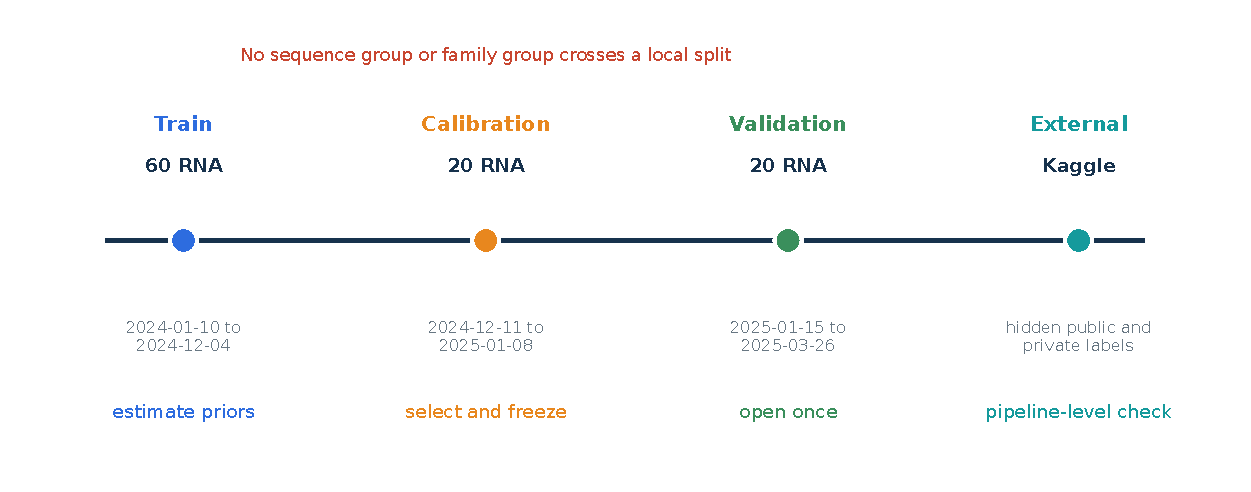
\includegraphics[width=0.96\textwidth]{evaluation_protocol.pdf}
\caption{Protocol bằng chứng hai tầng. Ba split local tách theo thời gian và họ; Kaggle
đóng vai trò external check ở mức toàn pipeline.}
\label{fig:evaluation_protocol_vi}
\end{figure}

Hình~\ref{fig:evaluation_protocol_vi} làm rõ thứ tự sử dụng dữ liệu. Các mũi tên thời
gian chỉ đi từ train sang calibration rồi validation; external leaderboard không quay
ngược vào quá trình chọn cấu hình. Đây là điều kiện quan trọng để diễn giải kết quả
private như kiểm tra ngoài mẫu thay vì một hyperparameter search khác.

\section{Cutoff thời gian và loại self-template}

Với target $q$ có cutoff $t_q$, template $s$ chỉ hợp lệ khi
\begin{equation}
\operatorname{release}(s) < t_q
\quad \text{và} \quad
\operatorname{PDB}(s) \notin \mathcal{E}_q,
\label{eq:temporal_gate_vi}
\end{equation}
trong đó $\mathcal{E}_q$ là tập PDB cần loại cho chính target. Bất đẳng thức nghiêm ngặt
tránh template phát hành đúng ngày cutoff đi qua do khác biệt múi giờ hoặc thứ tự cập
nhật. Nếu thiếu cutoff hay release date, một triển khai an toàn nên fail closed thay vì
coi template là hợp lệ.

Ảnh hưởng của leakage được minh họa trong Hình~\ref{fig:leakage_vi}. Trên pipeline CASP15
ban đầu, mean best-of-five TM tăng từ 0.1612 với temporal filter lên 0.6388 khi bỏ filter
và 0.9566 trong oracle leak. Các biến thể không an toàn không phải phương pháp cạnh
tranh; chúng chỉ định lượng mức lạc quan có thể xuất hiện nếu data snapshot không khớp
thời điểm đánh giá. Nguyên tắc benchmark mù của CASP và RNA-Puzzles cung cấp cơ sở cho
audit này \cite{rna_puzzles,casp15}.

\begin{figure}[H]
\centering
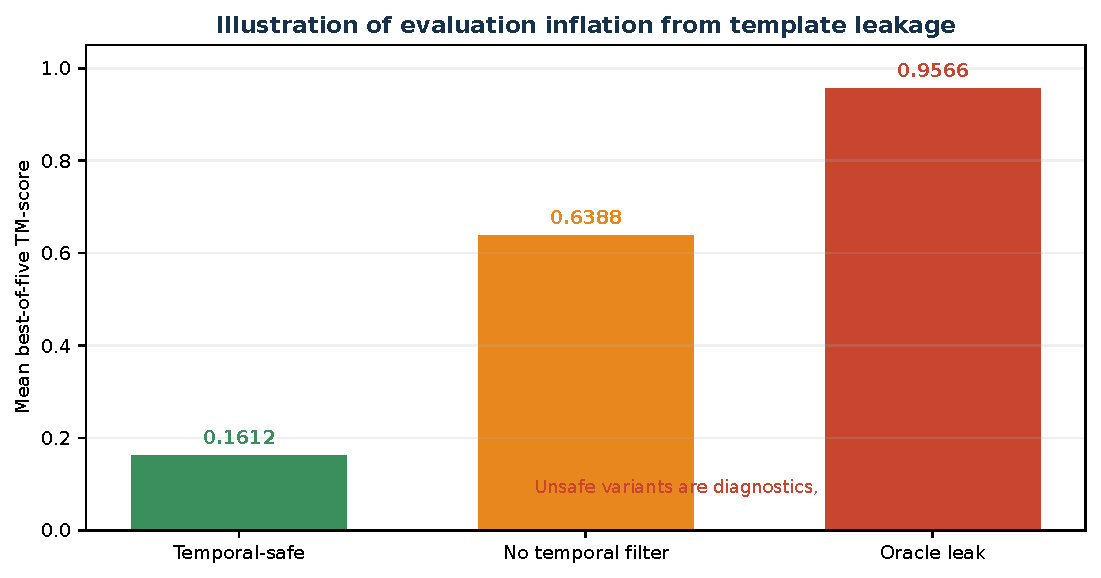
\includegraphics[width=0.77\textwidth]{leakage_diagnostic.pdf}
\caption{Minh họa mức tăng điểm do rò rỉ template trên cohort CASP15 phát triển. Hai cột
không an toàn chỉ là diagnostic và không tham gia kết quả phương pháp.}
\label{fig:leakage_vi}
\end{figure}

\section{Quy tắc sử dụng nhãn}

Native label chỉ được đọc trong các script đánh giá local sau khi candidate đã sinh.
Trong complementarity study, ``oracle'' nghĩa là phép lấy maximum dùng để đo trần có sẵn
của candidate bank; oracle không chọn cấu trúc trong pipeline inference. Geometry
refinement chỉ nhận tọa độ nguồn, confidence và prior từ train. Đối với mỗi candidate,
native conformation dùng khi tính local metric được cố định từ candidate raw để
refinement không hưởng lợi bằng cách đổi sang conformation tham chiếu dễ hơn.

Artifact Kaggle cuối không chứa validation label, hidden test label hay submission dựng
sẵn. Manifest ghi nhận \texttt{native\_labels\_used: false}; output có đúng 2,515 dòng,
18 cột, ID đúng thứ tự và tọa độ hữu hạn. SHA-256 của tệp cuối là
\begin{center}
\scriptsize\ttfamily 54fe6e6598a1c2924ef7cbf03482f7ecf3c2e52e8726a1609569f777b1ac8c9a
\end{center}
Các kiểm tra này chứng minh tính toàn vẹn của artifact triển khai, trong khi điều kiện ở
Phương trình~\ref{eq:temporal_gate_vi} kiểm soát tính hợp lệ của template.

\section{Đơn vị phân tích và thống kê}

Target RNA là đơn vị độc lập trong mọi khoảng tin cậy. Năm candidate của cùng target có
chung sequence, native và quá trình sinh, do đó không được xem như năm quan sát độc lập.
Với effect $d_i$ trên $n$ target, luận văn báo cáo
\begin{equation}
\bar d = \frac{1}{n}\sum_{i=1}^{n} d_i
\end{equation}
và khoảng tin cậy percentile từ 10,000 bootstrap sample lấy lại target có hoàn lại.
Bootstrap là phương pháp ước lượng độ bất định bằng resampling từ mẫu quan sát
\cite{bootstrap}. Seed được cố định ở 2025 để tái lập kết quả.

Một effect luôn được định hướng để giá trị dương nghĩa là tốt hơn. Với TM-score và lDDT,
$d_i=m_i^{\mathrm{new}}-m_i^{\mathrm{base}}$; với RMSD, clash hoặc deviation,
$d_i=m_i^{\mathrm{base}}-m_i^{\mathrm{new}}$. Quy ước này giúp các bảng có chung cách
đọc nhưng caption phải nêu rõ đơn vị. Luận văn báo cáo mean, median, khoảng tin cậy và số
target improve/tie/regress để tránh một trung bình che khuất failure case.

\chapter{Pipeline đề xuất}
\label{chap:method_vi}

\section{Tổng quan}

Pipeline nhận một RNA sequence và cutoff thời gian, sau đó sinh hai candidate bank độc
lập. Nhánh TBM trả tối đa ba cấu trúc đã xếp hạng; DRfold2 trả hai cấu trúc theo confidence
nội bộ. Nếu DRfold2 vượt giới hạn tài nguyên, vị trí còn thiếu được lấp bằng TBM. Geometry
refinement xử lý riêng từng candidate trong 300 bước và writer xuất đúng năm trace
\cprime{}. Hình~\ref{fig:pipeline_vi} tóm tắt luồng dữ liệu.

\begin{figure}[H]
\centering
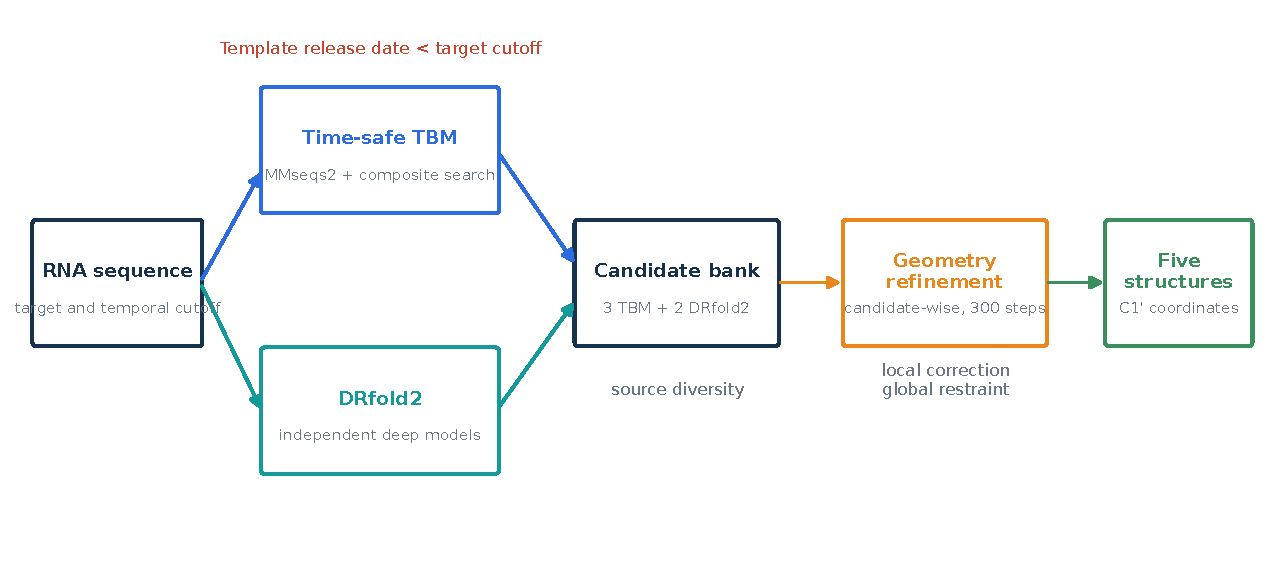
\includegraphics[width=\textwidth]{pipeline_overview.pdf}
\caption{Pipeline cuối. Đa dạng nguồn được tạo trước refinement; không có lựa chọn hay
hợp nhất tọa độ dựa trên native label.}
\label{fig:pipeline_vi}
\end{figure}

Thiết kế có hai nguyên tắc. Thứ nhất, diversity được tạo ở cấp nguồn bằng cách giữ ba
TBM và hai DRfold2, phù hợp với best-of-five evaluation. Thứ hai, refinement bị ràng
buộc gần source để tránh phá một fold vốn đã tốt. Hai nguyên tắc giải quyết hai failure
mode khác nhau và được đánh giá riêng ở Chương~\ref{chap:results_vi}.

\section{Nhánh TBM an toàn thời gian}

\subsection{Truy hồi hai đường}

Nhánh thứ nhất chạy MMseqs2 trên index sequence của template library. MMseqs2 dùng các
bộ lọc tăng tốc và căn chỉnh nhạy để xử lý cơ sở dữ liệu lớn
\cite{mmseqs2}. Raw hit được chuẩn hóa về chain key, identity, alignment coverage và
release date. Hit thiếu tọa độ \cprime{} hoặc vi phạm gate thời gian bị loại trước bước
xếp hạng.

Nhánh thứ hai quét thư viện sequence đã khử trùng lặp bằng điểm composite
\begin{equation}
S_{\mathrm{comp}}(q,s)=0.4G(q,s)+0.3L(q,s)+0.2F(q,s)+0.1K_3(q,s),
\label{eq:composite_vi}
\end{equation}
trong đó $G$ là global-alignment similarity, $L$ là local-alignment similarity, $F$ là
tương đồng đặc trưng thành phần và $K_3$ là overlap 3-mer. Global và local alignment
dựa trên hai quy hoạch động cổ điển \cite{needleman_wunsch,smith_waterman}. Các trọng số
trong Phương trình~\ref{eq:composite_vi} là heuristic frozen; ablation kiểm tra độ nhạy
thay vì gán cho chúng ý nghĩa xác suất.

\begin{figure}[H]
\centering
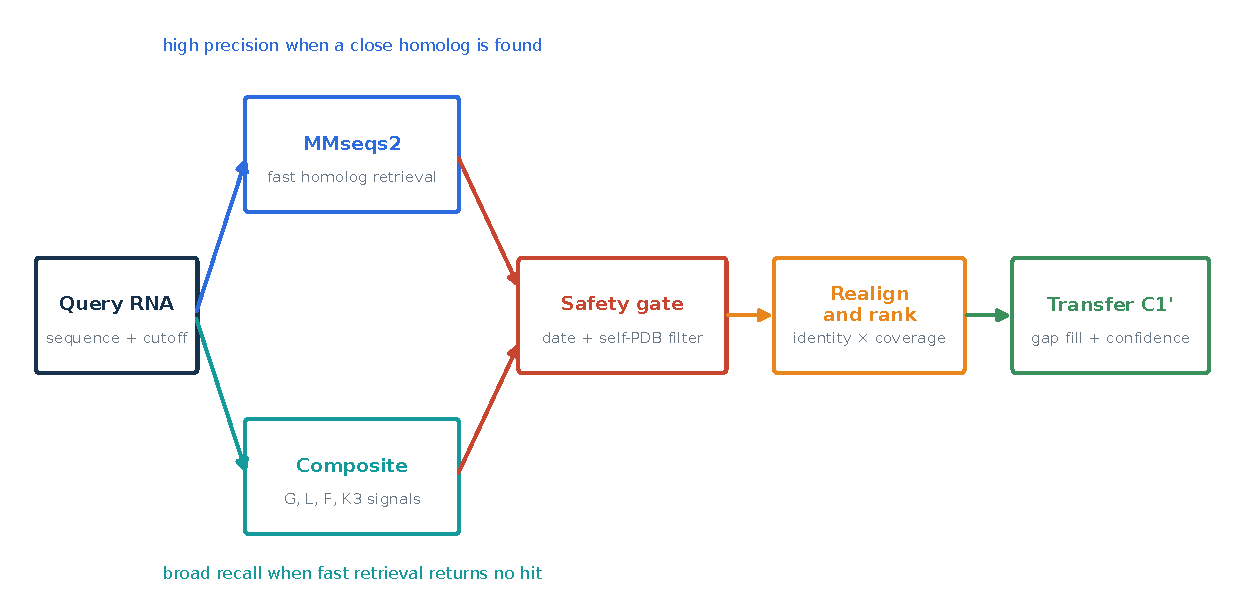
\includegraphics[width=0.98\textwidth]{tbm_flow.pdf}
\caption{Luồng TBM. MMseqs2 ưu tiên homolog rõ, composite mở rộng recall, còn safety gate
được áp dụng trước khi căn chỉnh lại và chuyển tọa độ.}
\label{fig:tbm_flow_vi}
\end{figure}

Hai danh sách được hợp nhất theo chain key trước khi lọc thời gian và self-PDB. Mẫu thiết
kế trong Hình~\ref{fig:tbm_flow_vi} giữ vai trò của hai search branch tách biệt: MMseqs2
không bị mô tả là kém khi nó không trả hit, còn composite không được coi là chính xác chỉ
vì nó luôn trả candidate. Availability và conditional quality được báo cáo riêng.

\subsection{Căn chỉnh lại và xếp hạng}

Mỗi hit hợp lệ được căn chỉnh toàn cục lại với query để tạo một hệ correspondence duy
nhất cho transfer. Gọi identity trên cột khớp là $I$, tỷ lệ query có tọa độ được hỗ trợ
là $C_q$ và completeness của template là $C_s$. Rank score được viết
\begin{equation}
S_{\mathrm{rank}} = I\,C_q\,C_s.
\label{eq:rank_vi}
\end{equation}
Trong pipeline cuối, identity nhân coverage tạo thứ tự chính; completeness dùng để xử
lý trường hợp tọa độ thiếu. Ba candidate đầu được ưu tiên từ PDB khác nhau khi có thể,
nhưng ablation kiểm tra riêng xem luật diversity này có tăng oracle TM trên cohort hay
không.

Điểm rank không phải confidence đã hiệu chỉnh. Nó là tín hiệu nội bộ để sắp thứ tự
candidate mà không nhìn native. Điểm này đặc biệt hữu ích khi một local hit có identity
cao nhưng chỉ phủ đoạn ngắn: nhân $C_q$ giảm khả năng hit đó chiếm vị trí đầu. Tác động
thực nghiệm của coverage được báo cáo ở Bảng~\ref{tab:tbm_rerank_vi}.

\subsection{Chuyển tọa độ và lấp khoảng trống}

Với mỗi cặp residue đã căn chỉnh, tọa độ \cprime{} của template được chép sang vị trí
query. Residue không được hỗ trợ được đánh dấu confidence thấp. Gap giữa hai anchor được
nội suy trên một đường cong xác định bởi hướng biên; terminal gap được ngoại suy từ các
bước backbone gần nhất. Nếu không có đủ anchor, pipeline dùng một trace de novo xác
định để bảo đảm output hữu hạn.

Curved gap filling chỉ nhằm tạo một candidate hợp lệ trước refinement. Nó không mang
thông tin native và không thể khôi phục một motif mới chỉ từ hai anchor. Vì vậy, thí
nghiệm chia gap theo độ dài và đo SW-RMSD9 tại residue không được hỗ trợ. Kết quả chỉ cho
thấy cải thiện rõ ở gap 9-20 nucleotide; các nhóm còn lại được báo cáo như kết quả trung
tính thay vì suy rộng.

\section{Nhánh DRfold2}

DRfold2 nhận sequence và sinh cấu trúc bằng một mô hình học sâu đã huấn luyện. Công
trình gốc mô tả một pipeline dự đoán RNA 3D hiệu quả và chính xác, phát triển từ DRfold
\cite{drfold,drfold2}. Luận văn giữ nguyên pretrained inference path và không fine-tune
bằng 100 RNA local. Hai model có confidence cao nhất được chuyển sang biểu diễn
$L\times3$ trên atom \cprime{}.

Các candidate DRfold2 được sinh độc lập với template hit. Độc lập ở đây nghĩa là nhánh
lựa chọn cuối không dùng native hoặc điểm TBM để uốn tọa độ DRfold2; nó không hàm ý tập
huấn luyện của pretrained model không có quan hệ với PDB. Audit mốc huấn luyện vì vậy
được ghi như một nguy cơ external validity, còn split theo họ bảo vệ thí nghiệm local
khỏi trùng lặp rõ ràng trong cohort dự án.

Giới hạn triển khai frozen là 600 nucleotide. Trong public execution, DRfold2 chạy cho
11/12 target và bỏ qua target 720 nucleotide; target đó giữ năm TBM. Luật fallback được
xác định trước khi chạy hidden set, nhờ đó output luôn có năm candidate mà không thay đổi
theo score.

\section{Geometry refinement}

\subsection{Mục tiêu thiết kế}

Cho candidate nguồn $X^{(0)}$, refinement tìm $X$ giảm một hàm mục tiêu hình học nhưng
không rời xa fold ban đầu. Mục tiêu tổng quát là
\begin{equation}
\mathcal{L}(X)=
\lambda_s\mathcal{L}_{\mathrm{source}}+
\lambda_b\mathcal{L}_{\mathrm{backbone}}+
\lambda_a\mathcal{L}_{\mathrm{angle}}+
\lambda_t\mathcal{L}_{\mathrm{torsion}}+
\lambda_c\mathcal{L}_{\mathrm{clash}}+
\lambda_k\mathcal{L}_{\mathrm{kink}}+
\lambda_r\mathcal{L}_{R_g}.
\label{eq:geometry_objective_vi}
\end{equation}
Mỗi hạng xử lý một failure mode, còn source term giới hạn drift. Hình
\ref{fig:refinement_mechanism_vi} minh họa cơ chế; đường vẽ mang tính khái niệm và không
phải một target thực nghiệm.

\begin{figure}[H]
\centering
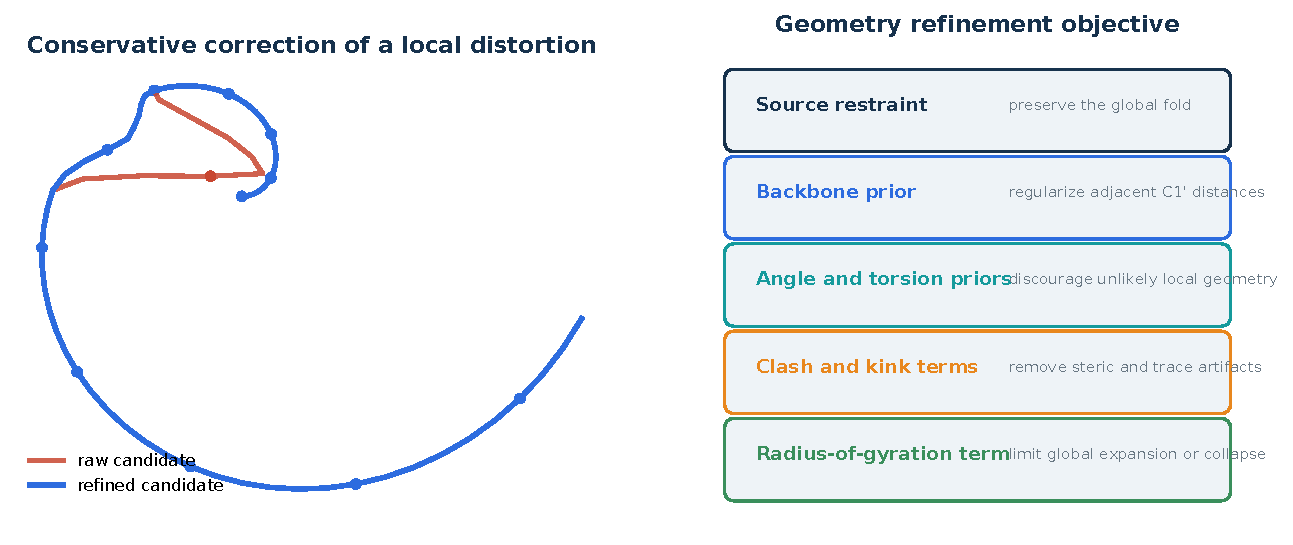
\includegraphics[width=0.98\textwidth]{refinement_mechanism.pdf}
\caption{Cơ chế geometry refinement. Một biến dạng cục bộ được làm trơn trong khi source
restraint bảo toàn bố cục tổng thể; các prior còn lại xử lý backbone, angle, torsion,
clash, kink và bán kính quán tính.}
\label{fig:refinement_mechanism_vi}
\end{figure}

\subsection{Prior hình học}

Khoảng cách kề nhau được ký hiệu $d_i=\lVert\mathbf{x}_{i+1}-\mathbf{x}_i\rVert_2$.
Trên 60 RNA train, phân bố này có mean 6.09~\angstrom{}, standard deviation
1.11~\angstrom{} và median 5.66~\angstrom{}. Ngưỡng clash \cprime{} không kề nhau được
đặt ở 4.18~\angstrom{}. Bán kính quán tính được mô hình bằng quan hệ power law
\begin{equation}
\widehat R_g(L)=5.18L^{0.346}.
\end{equation}
Các thống kê là prior của snapshot dự án, không phải hằng số vật lý phổ quát. Chúng được
ước lượng chỉ trên train và giữ cố định cho calibration cùng validation.

Backbone term sử dụng negative log-likelihood theo bin của $d_i$ và context cục bộ.
Angle term áp dụng cho bộ ba \cprime{} liên tiếp, torsion term cho bộ bốn liên tiếp. Kink
term phạt góc gập quá sắc, clash term phạt các cặp không kề nhau gần hơn ngưỡng, còn
$R_g$ term hạn chế collapse hoặc giãn quá mức. Các phân bố theo context cho phép trace
uốn tự nhiên hơn một target distance duy nhất.

Source restraint được điều chỉnh theo confidence:
\begin{equation}
\mathcal{L}_{\mathrm{source}}=
\frac{1}{L}\sum_{i=1}^{L}w_i
\lVert \mathbf{x}_i-\mathbf{x}^{(0)}_i\rVert_2^2,
\end{equation}
trong đó $w_i$ lớn hơn ở residue được template hỗ trợ hoặc có model confidence cao.
Thiết kế này cho phép gap và vùng yếu di chuyển nhiều hơn phần scaffold đáng tin. Toàn
bộ candidate được tối ưu 300 bước Adam với cấu hình \texttt{source\_1p5} đã khóa trên
calibration.

\subsection{Baseline và output}

Baseline đơn giản chỉ giữ source restraint và backbone smoothing. So sánh này trả lời
một câu hỏi thực tế: các term phức tạp có tạo lợi ích vượt một phép làm trơn bảo thủ hay
không? Full method phải được so với cả raw và baseline; thắng raw đơn thuần không đủ để
chứng minh mọi term cần thiết.

Sau refinement, mỗi candidate được kiểm tra shape $L\times3$, finite coordinates và thứ
tự residue. Writer ghép năm candidate thành các cột \texttt{x\_1,y\_1,z\_1} đến
\texttt{x\_5,y\_5,z\_5}, giữ đúng sample ID. Không có bước chọn source theo native,
không có coordinate fusion và không có mô hình router trong pipeline cuối.

\section{Mã giả}

\begin{enumerate}
  \item Nhận sequence $q$, cutoff $t_q$ và danh sách PDB cần loại.
  \item Truy hồi bằng MMseqs2 và composite; hợp nhất hit theo chain key.
  \item Loại hit không thỏa Phương trình~\ref{eq:temporal_gate_vi}.
  \item Căn chỉnh lại, tính rank score và tạo ba ứng viên TBM.
  \item Chạy DRfold2 nếu $L\leq600$ và giữ hai ứng viên theo model confidence.
  \item Nếu thiếu DRfold2, lấp slot bằng TBM; luôn tạo đúng năm candidate.
  \item Chạy geometry refinement độc lập trên từng candidate trong 300 bước.
  \item Kiểm tra ID, kích thước, thứ tự, uniqueness và finite coordinates; sau đó ghi CSV.
\end{enumerate}

Mã giả cho thấy native label không nằm trên inference path. Tất cả quyết định trước khi
ghi output dựa trên sequence, template metadata, pretrained confidence và prior aggregate.
Điều này tách selection blind khỏi oracle score chỉ được tính trong bước đánh giá.

\chapter{Thiết kế thí nghiệm}
\label{chap:experiment_vi}

\section{Chiến lược kiểm định}

Mỗi RQ được gắn với một nhóm thí nghiệm và một claim tối đa. RQ1 dùng 20 RNA calibration
để mổ search source, composite score, reranking và gap fill. RQ2 dùng 20 RNA validation
để so candidate bank trước refinement. RQ3 dùng protocol 60/20/20, trong đó validation
chỉ được mở sau khi khóa cấu hình. Phân tách này ngăn kết quả khám phá TBM trở thành bằng
chứng xác nhận cho geometry refinement.

\begin{table}[H]
\centering
\caption{Ánh xạ câu hỏi nghiên cứu sang thí nghiệm và claim.}
\label{tab:rq_map_vi}
\begin{tabularx}{\textwidth}{p{1.0cm}X X}
\toprule
RQ & So sánh chính & Claim được phép \\
\midrule
RQ1 & MMseqs2, composite, union; component và reranking ablation & Composite mở rộng availability; hiệu quả ranking được định lượng theo thành phần \\
RQ2 & 3T, 2D, union; fixed-N allocation & TBM và DRfold2 bổ sung nhau theo target \\
RQ3 & Raw, source+backbone, full refinement; cumulative và leave-one-out & Refinement cải thiện local trace trong biên bảo toàn TM \\
\bottomrule
\end{tabularx}
\end{table}

Bảng~\ref{tab:rq_map_vi} giới hạn mức diễn giải trước khi nhìn kết quả. Đặc biệt, RQ3
không đặt giả thuyết tăng TM-score. Hệ thống có thể đạt validation gate nếu local metric
cải thiện và mean TM change nằm trong biên $\pm0.005$. Biên được khóa trên calibration
để tránh thay đổi tiêu chí sau khi mở validation.

\section{Ablation TBM}

Search-source study so sánh ba cấu hình: MMseqs2-only, composite-only và union. Với
MMseqs2, TM chỉ được tính có điều kiện trên target có hit, đồng thời availability được
báo riêng. Với composite và union, mean tính trên đủ 20 target. Cách báo cáo này tránh
so sánh 8 target dễ với 20 target đầy đủ như thể hai mẫu giống nhau.

Composite component study so sánh $G$, $G+L$, $G+L+F$, tổ hợp bốn thành phần trọng số
bằng nhau, full weighted và các biến thể đổi từng trọng số $\pm25\%$. Tập hit chung được
dùng để tính useful recall ở ngưỡng TM 0.45; đại lượng này là diagnostic nội bộ, không
phải metric chính thức. Temporal-unsafe variant chỉ lượng hóa leakage.

Reranking study bắt đầu từ identity-only rồi lần lượt thêm query coverage, template
completeness và distinct-PDB selection. Gap study so linear với curved interpolation ở
bốn nhóm độ dài 1-3, 4-8, 9-20 và trên 20 nucleotide. Mỗi gap được đo tại residue không
có template support; các gap trong cùng target được trung bình trước target bootstrap.

\section{Thí nghiệm tính bổ sung}

Candidate source được đánh giá trước geometry refinement để không trộn hai factor. Với
target $i$, đặt $T_i$ là ba TBM score và $D_i$ là hai DRfold2 score. Ba oracle statistic
là
\begin{equation}
O_T(i)=\max T_i,\quad O_D(i)=\max D_i,\quad
O_U(i)=\max(T_i\cup D_i).
\end{equation}
Union gain $O_U-O_T$ đo giá trị tối đa sẵn có khi thêm hai candidate DRfold2. Vì
$|T_i\cup D_i|>|T_i|$, phép đo này bao gồm cả source diversity và candidate-count effect.

Để kiểm soát số slot, fixed-N=2 so $2T$ với $1T+1D$, còn fixed-N=3 so $3T$ với
$2T+1D$. Candidate trong mỗi nguồn được chọn bằng thứ tự confidence blind. Cache chỉ có
ba TBM và hai DRfold2 cho mỗi RNA, nên không thể dựng một sweep đủ từ $5T$ đến $5D$ mà
không nhân bản candidate. Luận văn báo giới hạn này thay vì tạo một allocation giả.

\section{Thí nghiệm geometry refinement}

Train split chỉ ước lượng prior. Trên calibration, cumulative ablation thêm lần lượt
source, backbone, angle, torsion, clash, kink và $R_g$; leave-one-out bỏ từng term khỏi
full objective. Cấu hình \texttt{source\_1p5} được chọn vì đạt local gain trong khi thỏa
TM preservation gate, sau đó được serialize trước validation.

Validation so ba setting: raw, simple source+backbone và full refinement. Primary local
metrics là \cprime{}-lDDT, SW-RMSD9 và SW-RMSD15. Global safeguard là best-of-five
TM-score; C1 RMSD toàn cấu trúc và SW-RMSD31 là secondary. Backbone deviation, clash,
sharp kink, angle-NLL, torsion-NLL và $R_g$ error chỉ là mechanism diagnostics vì chúng
nằm trong hoặc gần objective.

Factorial fixed-N=3 tạo bốn cell: $3T$ raw, $3T$ refined, $2T+1D$ raw và $2T+1D$
refined. Main effects ước lượng source-bank gain khi refinement off và geometry effect
trong từng bank. Interaction kiểm tra refinement có hoạt động khác theo source composition
hay không. Thiết kế này trực tiếp kiểm tra liệu geometry refinement có thể giải thích
mức tăng TM của pipeline hybrid.

\section{External evaluation và khả năng tái lập}

Hai submission frozen được so sánh: time-safe composite TBM và pipeline cuối. Submission
TBM chạy search, rank, transfer, gap fill và refinement của baseline hiện có; submission
hybrid thay hai slot bằng DRfold2 khi khả thi rồi áp dụng cấu hình geometry refinement đã
khóa. Public và private score được đọc từ Kaggle, còn integrity được kiểm tra từ manifest
và output hash \cite{kaggle_competition}.

Mọi bảng local được tạo bởi script trong repository. Random seed của bootstrap là 2025;
cấu hình, prior provenance và candidate cache được lưu cùng artifact. Các phép kiểm tra
bao gồm một target mỗi dòng trong metadata, không có group crossing split, đúng ba TBM
và hai DRfold2 mỗi target, tọa độ hữu hạn và không thay đổi native conformation giữa raw
với refined evaluation. Danh sách tệp tái lập được ghi ở Phụ lục~\ref{app:repro_vi}.

\chapter{Kết quả}
\label{chap:results_vi}

\section{RQ1: Truy hồi và xếp hạng TBM}

\subsection{Hai nguồn truy hồi}

MMseqs2 tìm được template cho 8/20 RNA calibration, tương ứng availability 40\%. Trên
riêng tám target có hit, top-1 TM là 0.660029 và best-of-five TM là 0.678316. Composite
search tạo candidate cho 20/20 target nhưng best-of-five mean chỉ 0.376060. Union giữ
availability 100\% và tăng mean lên 0.389705. Bảng~\ref{tab:search_source_vi} trình bày
đầy đủ ba đại lượng.

\begin{table}[H]
\centering
\caption{Ảnh hưởng của nguồn truy hồi trên 20 RNA calibration. Điểm MMseqs2 là conditional
trên tám target có hit.}
\label{tab:search_source_vi}
\resizebox{\textwidth}{!}{%
\begin{tabular}{lrrr}
\toprule
Nguồn & Target có hit & Availability & Best-of-five TM khi có hit \\
\midrule
MMseqs2-only & 8/20 & 0.40 & 0.678316 \\
Composite-only & 20/20 & 1.00 & 0.376060 \\
MMseqs2 + composite & 20/20 & 1.00 & 0.389705 \\
\bottomrule
\end{tabular}
}
\end{table}

Kết quả cho thấy hai search branch có vai trò khác nhau. Khi MMseqs2 nhận ra homolog,
candidate thường mạnh; composite lấp 12 target còn thiếu nhưng precision trung bình thấp
hơn. Union tăng 0.013645 so với composite-only, song khoảng tin cậy
$[-0.004417,0.042781]$ chứa 0 vì chỉ hai target thay đổi theo chiều tốt. Do đó, lợi ích
được hỗ trợ rõ nhất là availability, không phải superiority trung bình của mọi composite
hit.

\subsection{Thành phần composite}

Full weighted đạt best-of-five TM 0.376060, trong khi G-only đạt 0.381177. Chênh lệch
theo chiều G-only tốt hơn là 0.005117 với khoảng tin cậy
$[-0.002178,0.015004]$. Các biến thể đổi trọng số $\pm25\%$ nằm trong khoảng
0.375436-0.376500. Như vậy, công thức composite ổn định trước nhiễu nhỏ nhưng không có
bằng chứng rằng bốn thành phần vượt global alignment trên cohort này.

Tuy vậy, $G+L+F$ có useful recall 0.676304 so với 0.635488 của G-only trong tập hit chung.
Mẫu này phù hợp với vai trò recall heuristic: tín hiệu bổ sung có thể đưa candidate mới
vào top five dù mean oracle chưa tăng rõ. Vì useful recall dùng threshold nội bộ, luận
văn không dùng nó thay thế TM-score.

Bỏ temporal filter làm mean tăng từ 0.376060 lên 0.403022, chênh 0.026962. Khoảng tin
cậy $[-0.000343,0.071258]$ còn rộng và 15/20 target không đổi. Kết quả không chứng minh
unsafe search tốt hơn; nó cho thấy chỉ một vài leaked template cũng đủ dịch chuyển mean
và vì vậy time filter là yêu cầu về tính hợp lệ.

\subsection{Reranking và gap fill}

Thêm query coverage vào identity tăng top-five TM từ 0.371900 lên 0.387558, tương ứng
$+0.015659$ với khoảng tin cậy $[-0.003731,0.045178]$. Thêm completeness không đổi
điểm trên cohort này; distinct-PDB selection cũng giữ nguyên oracle TM dù số PDB riêng
trung bình tăng từ 4.95 lên 5.00. Bảng~\ref{tab:tbm_rerank_vi} cho thấy dominant pattern
là coverage, còn hai rule sau chủ yếu bảo vệ robustness và diversity.

\begin{table}[H]
\centering
\caption{Ablation xếp hạng TBM.}
\label{tab:tbm_rerank_vi}
\begin{tabular}{lrrr}
\toprule
Xếp hạng & Top-1 TM & Top-3 TM & Top-5 TM \\
\midrule
Identity only & 0.334450 & 0.363854 & 0.371900 \\
Identity $\times$ coverage & 0.363720 & 0.378412 & 0.387558 \\
$+\,$template completeness & 0.363720 & 0.378412 & 0.387558 \\
$+\,$distinct PDB & 0.363720 & 0.378412 & 0.387558 \\
\bottomrule
\end{tabular}
\end{table}

Curved gap filling chỉ cải thiện rõ ở gap dài 9-20 nucleotide. SW-RMSD9 giảm trung bình
0.036778~\angstrom{} với khoảng tin cậy $[0.009289,0.067605]$. Gap 1-3 và 4-8 không có
bằng chứng khác linear interpolation, còn gap trên 20 không đổi trong triển khai hiện
tại. Cơ chế hợp lý là đường cong có đủ chiều dài để tránh đoạn nối thẳng, nhưng hai
anchor vẫn không đủ thông tin cho gap rất dài.

\section{RQ2: TBM và DRfold2 bổ sung nhau}

Trước refinement, ba TBM đạt mean oracle 0.565183 và hai DRfold2 đạt 0.502627. Union năm
candidate đạt 0.588304, cao hơn TBM 0.023121 với khoảng tin cậy
$[0.006444,0.047519]$. DRfold2 cung cấp candidate tốt nhất ở 8/20 target, còn TBM thắng
ở 12/20. Hình~\ref{fig:complementarity_vi} cho thấy cả mức điểm và winner count.

\begin{figure}[H]
\centering
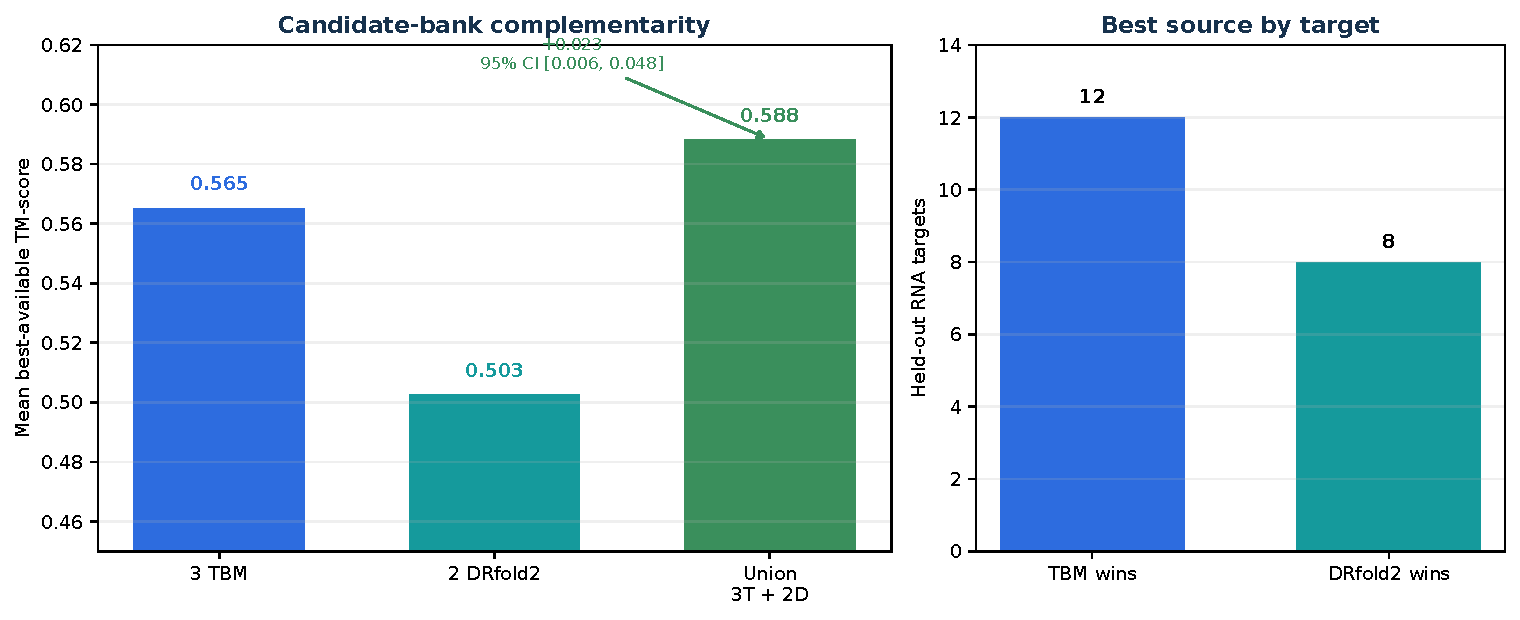
\includegraphics[width=0.92\textwidth]{complementarity_results.pdf}
\caption{Tính bổ sung của candidate bank trên 20 RNA validation. Union gain được tính so
với ba TBM và khoảng tin cậy bootstrap theo target.}
\label{fig:complementarity_vi}
\end{figure}

Kết quả chính không phải DRfold2 có mean cao hơn TBM; thực tế mean của nhánh học sâu thấp
hơn 0.062556. Giá trị nằm ở tám target mà thứ tự nguồn đảo chiều. Vì oracle union không
thể giảm khi thêm candidate, fixed-N là đối chứng cần thiết để xác định effect không chỉ
do hai slot mới.

Với hai slot, $1T+1D$ cao hơn $2T$ trung bình 0.030546, khoảng tin cậy
$[0.002949,0.068185]$. Với ba slot, $2T+1D$ cao hơn $3T$ 0.016012, nhưng khoảng tin cậy
$[-0.002072,0.041466]$ chứa 0 và mười target hòa. Mẫu giảm effect theo số TBM cho thấy
candidate DRfold2 có giá trị lớn nhất khi nó thay một template dư thừa; khi ba TBM đã đa
dạng, lợi ích biên nhỏ hơn và bất định hơn.

\begin{table}[H]
\centering
\caption{Candidate allocation với geometry refinement tắt.}
\label{tab:allocation_vi}
\resizebox{\textwidth}{!}{%
\begin{tabular}{lrrl}
\toprule
So sánh & Mean baseline & Mean hybrid & Mean gain và CI 95\% \\
\midrule
$2T$ so với $1T+1D$ & 0.549040 & 0.579586 & $+0.030546$ $[0.002949,0.068185]$ \\
$3T$ so với $2T+1D$ & 0.565183 & 0.581196 & $+0.016012$ $[-0.002072,0.041466]$ \\
$3T$ so với $3T+2D$ & 0.565183 & 0.588304 & $+0.023121$ $[0.006444,0.047519]$ \\
\bottomrule
\end{tabular}
}
\end{table}

Bảng~\ref{tab:allocation_vi} phân biệt fixed-size effect và production-bank effect.
Dòng $3T+2D$ mô tả trần sẵn có của pipeline năm slot; hai dòng fixed-N kiểm tra fairness.
Ở cả $N=2$ và $N=3$, thay một TBM bằng một DRfold2 làm mean tăng, nhưng chỉ khoảng tin
cậy của so sánh hai slot nằm hoàn toàn phía dương.

\section{RQ3: Geometry refinement}

\subsection{Kết quả xác nhận}

Full refinement tăng \cprime{}-lDDT từ 0.659836 lên 0.666496, tương ứng
$+0.006660$ với khoảng tin cậy $[0.000933,0.013093]$; 12/20 target cải thiện. SW-RMSD9
giảm từ 2.651395 xuống 2.611010~\angstrom{}, mức tốt lên 0.040386~\angstrom{} với
khoảng tin cậy $[0.029354,0.052090]$ và 19/20 target cải thiện. SW-RMSD15 giảm
0.017257~\angstrom{}, khoảng tin cậy $[0.000617,0.031336]$, tốt hơn ở 15/20 target.

Global TM thay đổi từ 0.588304 xuống 0.587197, tức $-0.001107$ với khoảng tin cậy
$[-0.002809,0.000418]$. Effect nằm trong biên bảo toàn 0.005 đã khóa. C1 RMSD toàn cấu
trúc và SW-RMSD31 chưa có bằng chứng thay đổi. Hình~\ref{fig:geometry_results_vi} cho
thấy local improvement cùng global preservation trong hai panel có đơn vị riêng.

\begin{figure}[H]
\centering
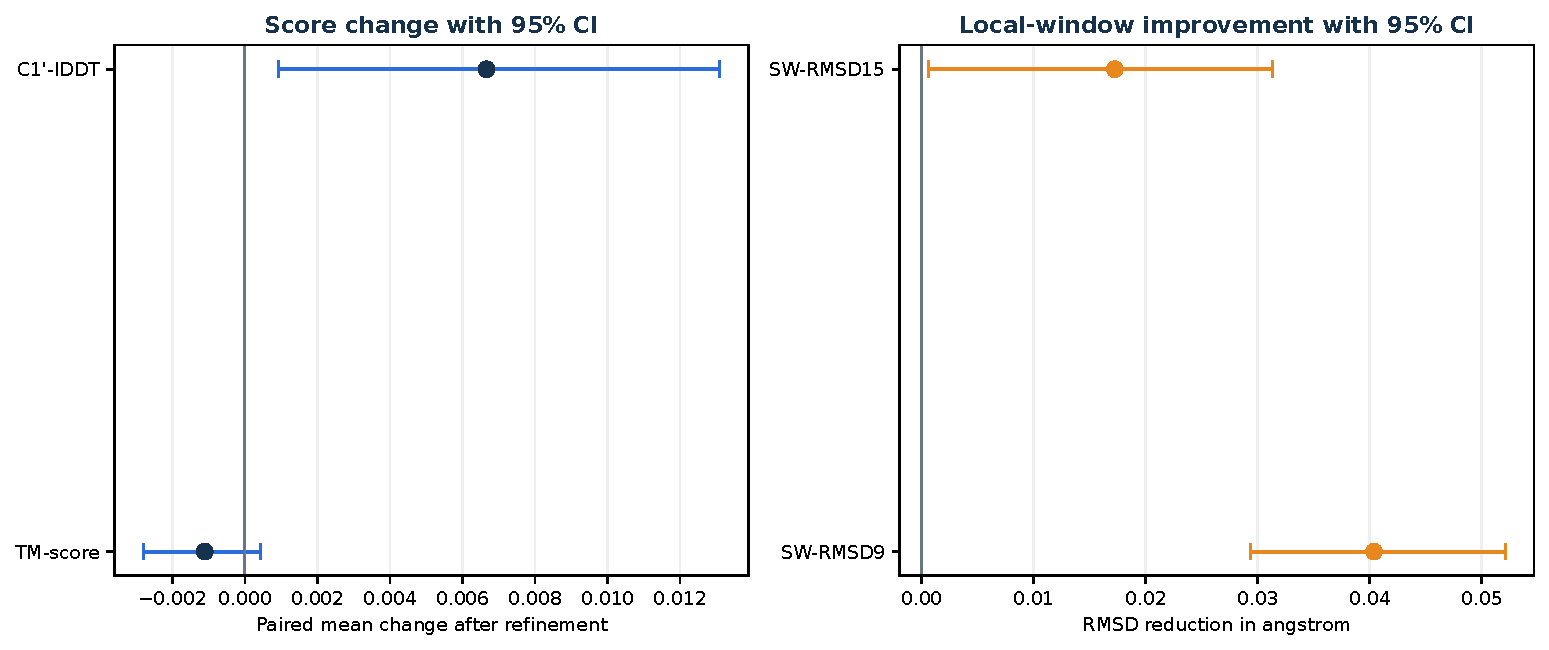
\includegraphics[width=0.94\textwidth]{geometry_results.pdf}
\caption{Effect confirmatory của geometry refinement. Điểm tăng dùng trục score; RMSD
reduction dùng angstrom và được định hướng dương là tốt hơn.}
\label{fig:geometry_results_vi}
\end{figure}

\begin{table}[H]
\centering
\caption{Raw và full geometry refinement trên 20 RNA validation.}
\label{tab:geometry_main_vi}
\resizebox{\textwidth}{!}{%
\begin{tabular}{lrrrl}
\toprule
Metric & Raw & Refined & Thay đổi tốt lên & CI 95\% \\
\midrule
Best-of-five TM & 0.588304 & 0.587197 & $-0.001107$ & $[-0.002809,0.000418]$ \\
\cprime{}-lDDT & 0.659836 & 0.666496 & $+0.006660$ & $[0.000933,0.013093]$ \\
SW-RMSD9 (\angstrom{}) & 2.651395 & 2.611010 & $+0.040386$ & $[0.029354,0.052090]$ \\
SW-RMSD15 (\angstrom{}) & 4.273393 & 4.256136 & $+0.017257$ & $[0.000617,0.031336]$ \\
Backbone deviation (\angstrom{}) & 1.040270 & 0.785817 & $+0.254453$ & diagnostic \\
Clash per residue & 0.065121 & 0.022802 & $+0.042319$ & diagnostic \\
\bottomrule
\end{tabular}
}
\end{table}

Dominant pattern trong Bảng~\ref{tab:geometry_main_vi} là hiệu quả tăng khi metric tập
trung vào cửa sổ ngắn. SW-RMSD9 có effect ổn định nhất, SW-RMSD15 nhỏ hơn, còn SW-RMSD31
và global RMSD không rõ. Gradient theo scale này khớp với mục tiêu thiết kế: refinement
di chuyển quan hệ lân cận chứ không tái sắp xếp toàn fold.

\subsection{Baseline đơn giản và ablation}

Source+backbone baseline tăng lDDT 0.007581, cao hơn numeric gain 0.006660 của full
method. Chênh full trừ simple là $-0.000921$ với khoảng tin cậy
$[-0.003118,0.001327]$, do đó full objective không được xem là vượt baseline về lDDT.
Ngược lại, full method giảm SW-RMSD9 thêm 0.030585~\angstrom{} so với simple, khoảng tin
cậy $[0.019640,0.044115]$, và sửa angle-NLL, torsion-NLL, clash cùng kink mà baseline
đơn giản làm xấu.

Leave-one-out trên calibration liên kết từng term với cơ chế. Bỏ backbone gần như làm
mất lDDT gain; bỏ angle hoặc torsion làm xấu NLL tương ứng; bỏ kink tăng sharp-kink rate;
bỏ clash hoặc $R_g$ làm clash diagnostic xấu. Các kết quả này chứng minh objective hoạt
động theo thiết kế, nhưng không biến diagnostic đã tối ưu thành bằng chứng độc lập. Claim
chính vẫn dựa trên lDDT và sliding-window RMSD.

\subsection{Factorial source và refinement}

Trên bank $3T$, refinement làm TM thay đổi $-0.005852$ với khoảng tin cậy
$[-0.014781,0.000724]$. Trên bank $2T+1D$, effect là $-0.002604$ với khoảng tin cậy
$[-0.005473,-0.000278]$. Interaction bằng $+0.003248$ và khoảng tin cậy chứa 0. Bảng
\ref{tab:factorial_vi} cho thấy source-bank effect dương khi geometry tắt, trong khi
geometry effect không dương ở cả hai bank.

\begin{table}[H]
\centering
\caption{Factorial fixed-N=3 tách source composition và geometry refinement.}
\label{tab:factorial_vi}
\begin{tabular}{lrr}
\toprule
Candidate bank & Raw mean TM & Refined mean TM \\
\midrule
$3T+0D$ & 0.565183 & 0.559331 \\
$2T+1D$ & 0.581196 & 0.578592 \\
\bottomrule
\end{tabular}
\end{table}

Factorial bác bỏ cách giải thích đơn giản rằng refinement tạo ra mức tăng global TM của
pipeline hybrid. Khi geometry tắt, đổi từ $3T$ sang $2T+1D$ đã tạo mean gain 0.016012.
Khi bật geometry, cả hai bank giảm nhẹ về TM. Kết quả cùng complementarity study ủng hộ
source diversity là cơ chế global chính; geometry refinement cung cấp một effect local
khác hướng đo.

\subsection{Phân tầng và failure case}

Phân tích hậu kiểm cho thấy candidate có chất lượng ban đầu thấp tăng lDDT 0.016261,
khoảng tin cậy $[0.008900,0.024089]$. Nhóm chất lượng cao thay đổi $-0.001788$ với
khoảng tin cậy $[-0.005775,0.002420]$. Pattern gợi ý source restraint cố định có thể quá
mạnh cho candidate yếu hoặc refinement không cần thiết cho candidate đã tốt. Vì nhóm
được định nghĩa sau khi mở validation, kết quả chỉ tạo giả thuyết cho quality gate tương
lai.

Ba failure case cần được giữ trong narrative. Target \texttt{9E2Z\_F} và
\texttt{8K7W\_A} giảm TM khoảng 0.009; \texttt{9B0S\_Et} giảm lDDT khoảng 0.011.
Refinement bảo thủ vì vậy không đồng nghĩa với monotonic improvement trên từng target.
Khoảng tin cậy trung bình và số improve/regress cùng cần thiết để phản ánh rủi ro này.

\section{Đánh giá external trên Kaggle}

Time-safe composite TBM đạt 0.60084 public và 0.60175 private. Pipeline cuối đạt
0.62809 public và 0.61390 private, tương ứng tăng 0.02725 và 0.01215. Notebook TBM-only
tham chiếu báo private 0.59298 \cite{kaggle_top1}; pipeline cuối cao hơn mốc này 0.02092.
Hình~\ref{fig:leaderboard_vi} đặt ba kết quả trên cùng thang đo.

\begin{figure}[H]
\centering
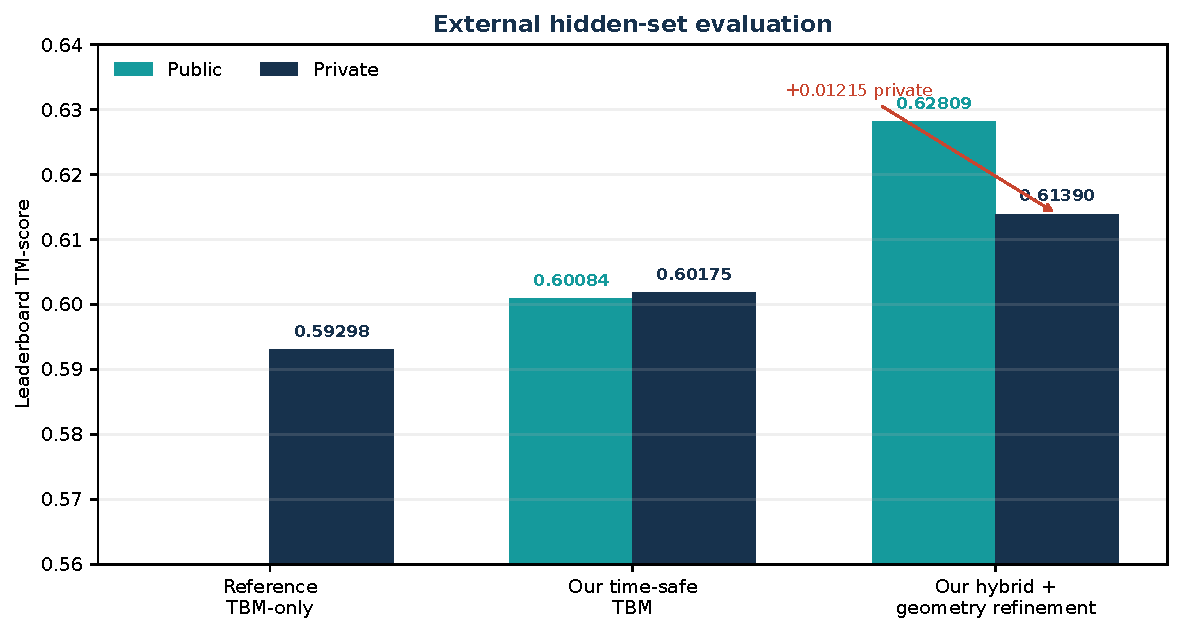
\includegraphics[width=0.86\textwidth]{leaderboard_results.pdf}
\caption{Đánh giá hidden-set. Mốc TBM-only tham chiếu chỉ có private score được báo cáo;
hai phương pháp của luận văn có cả public và private score.}
\label{fig:leaderboard_vi}
\end{figure}

Public execution cung cấp sanity check cho deployment. DRfold2 sinh hai candidate ở
11/12 target; target 720 nucleotide dùng năm TBM do resource limit. Geometry refinement
hoàn tất cho 60/60 candidate, output có đúng schema và không đọc native. Những kiểm tra
này hỗ trợ tính tin cậy của điểm nhưng không cho biết target hidden nào tạo mức tăng.

Kết quả Kaggle phải được đọc cùng local factorial. Lần nộp cuối thay hai TBM slot bằng
DRfold2 và áp dụng refinement, nên $+0.01215$ private là pipeline-level effect. Local
evidence cho thấy hybrid bank tăng global TM trước refinement, trong khi refinement cải
thiện local metric và làm TM giảm nhẹ. Sự kết hợp hai nguồn bằng chứng giải thích vì sao
pipeline vượt mốc tham chiếu mà không gán toàn bộ chênh lệch cho geometry refinement.

\begin{figure}[H]
\centering
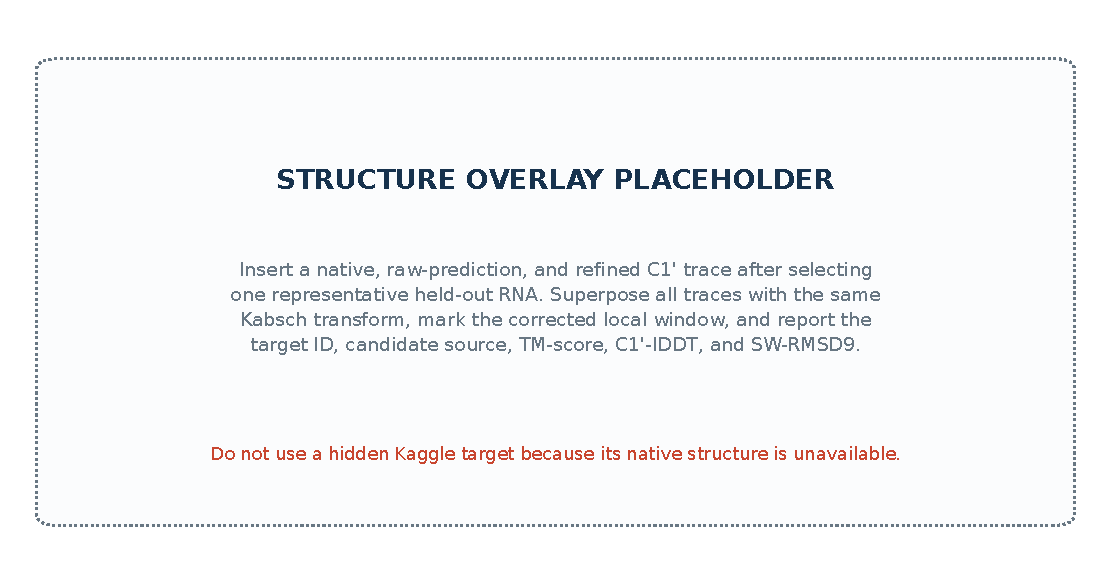
\includegraphics[width=0.88\textwidth]{structure_overlay_placeholder.pdf}
\caption{Placeholder cho hình chồng cấu trúc. Bản cuối nên dùng một RNA validation có
native công khai, cùng một Kabsch transform và đầy đủ provenance; không dùng target
hidden Kaggle.}
\label{fig:overlay_placeholder_vi}
\end{figure}

Hình~\ref{fig:overlay_placeholder_vi} được giữ có chủ ý thay vì dựng một minh họa giả.
Khi chọn target đại diện, tiêu chí nên được khai báo trước, chẳng hạn target có SW-RMSD9
gần median effect. Caption cuối cần ghi target ID, candidate source, raw và refined
metric, cửa sổ được đánh dấu cùng script tạo hình.

\chapter{Thảo luận}
\label{chap:discussion_vi}

\section{Vì sao pipeline hybrid có giá trị}

Kết quả vượt mốc TBM-only không xuất phát từ việc một nhánh luôn mạnh hơn nhánh kia. TBM
có mean oracle cao hơn DRfold2 và thắng 12/20 target, nhưng DRfold2 thắng tám target còn
lại. Khi metric lấy best-of-five, một candidate nguồn khác chỉ cần thắng ở một tập con
đủ lớn để nâng mean union. Complementarity vì vậy là thuộc tính phân bố theo target, không
phải chênh lệch mean của từng source.

Fixed-N=2 củng cố lập luận bằng cách loại candidate-count advantage: thay một trong hai
TBM bằng DRfold2 vẫn tạo gain có khoảng tin cậy dương. Fixed-N=3 yếu hơn vì ba TBM đã giữ
nhiều diversity hơn và cohort chỉ có 20 target. Cùng với union gain dương, pattern này
cho thấy allocation ba TBM và hai DRfold2 là một thỏa hiệp hợp lý cho hidden distribution,
không phải tỷ lệ phổ quát cho mọi benchmark.

TBM mạnh trong cuộc thi còn có một nguyên nhân dữ liệu. Paper tổng kết cho biết 19/20
private target có ít nhất một prior structure với TM-align trên 0.45, cao hơn tỷ lệ của
CASP15 \cite{competition_paper}. Snapshot template lớn và composite search giúp pipeline
khai thác regime giàu khuôn này. Tuy nhiên, chính paper cũng cảnh báo kết luận ưu tiên TBM
có thể không khái quát sang template-poor RNA \cite{competition_paper}. DRfold2 giữ giá
trị như bảo hiểm cho phần phân bố đó.

\section{Vì sao geometry refinement không tăng TM-score}

Source restraint làm objective có một nghiệm gần candidate đầu. Backbone, angle, torsion
và clash term chủ yếu tác động trên quan hệ ngắn hạn; chúng không cung cấp tín hiệu để
đổi topology hoặc dịch chuyển cả domain. Do đó, lDDT và SW-RMSD9 cải thiện trong khi TM
gần như giữ nguyên là kết quả phù hợp với thiết kế, không phải mâu thuẫn.

Một global fold sai cần thông tin về contact xa, motif hoặc template khác. Tối ưu một
trace quanh source không thể tự tạo thông tin này. Quan sát tương tự đã được thảo luận
trong refinement nucleic acid: cải thiện stereochemistry không bảo đảm systematic RMSD
improvement \cite{qrnas}. Vì vậy, geometry refinement nên được xem như hậu xử lý chất
lượng hình học, còn source diversity quyết định trần global chính.

Simple baseline tăng lDDT ngang full method, cho thấy backbone smoothing là cơ chế mạnh
nhất cho metric này. Giá trị bổ sung của full objective xuất hiện rõ hơn ở SW-RMSD9 và
các diagnostic angle, torsion, clash, kink. Điều này thu hẹp contribution: full method
không cần thiết để đạt mọi local gain, nhưng nó tạo một trace cân bằng hơn trên nhiều
ràng buộc mà không phá global fold trung bình.

\section{Diễn giải điểm leaderboard}

Điểm private 0.61390 có value vì được đo trên cấu trúc ẩn và cao hơn cả pipeline TBM của
dự án lẫn mốc notebook tham chiếu. Nó chứng minh implementation đầy đủ hoạt động trên
một phân bố ngoài cohort local. Tuy nhiên, một scalar score không chứa per-target
counterfactual. Không thể biết cùng target sẽ đạt bao nhiêu nếu chỉ tắt refinement hoặc
đổi một slot DRfold2 sau khi cuộc thi đã đóng.

Lập luận thuyết phục vì thế gồm ba lớp. Thứ nhất, integrity audit cho thấy submission
không dùng native và tuân temporal gate. Thứ hai, local complementarity xác định một
cơ chế global có effect dương. Thứ ba, local refinement xác định một cơ chế local riêng
và cho thấy nó không tăng TM. Ba lớp cùng giải thích kết quả nhưng vẫn giữ ranh giới giữa
external performance và component causality.

Sự đảo chiều giữa cohort cũng đáng chú ý. Rule frozen trên 12 CASP15 target đạt 0.46450
và kém local TBM bank, trong khi private Kaggle tăng 0.01215. Khác biệt cho thấy target
distribution quyết định allocation hiệu quả. Báo cáo cả hai kết quả đáng tin cậy hơn
việc chọn cohort thuận lợi, đồng thời phản bác claim rằng một tỷ lệ nguồn luôn tối ưu.

\section{Nguy cơ đối với tính hợp lệ}

\subsection{Tính hợp lệ nội tại}

Calibration và validation chỉ có 20 target mỗi split, vì vậy interval còn rộng cho nhiều
ablation. Bootstrap theo target xử lý dependence giữa candidate nhưng không tạo thêm
thông tin ngoài 20 RNA \cite{bootstrap}. Nhiều phân tích subgroup làm tăng khả năng tìm
thấy pattern ngẫu nhiên; luận văn do đó ghi chúng là post hoc và không dùng để thay đổi
method.

Candidate cache chỉ có ba TBM và hai DRfold2. Fixed-N đến ba slot được xác định đầy đủ,
nhưng allocation năm slot từ $5T$ đến $5D$ không thể đánh giá. Một nghiên cứu tiếp theo
cần sinh ít nhất năm candidate độc lập từ mỗi nguồn trước khi mở cohort mới.

\subsection{Tính hợp lệ external}

Validation local dài tối đa 96 nucleotide và tập trung vào RNA đơn chuỗi. Kết quả
refinement không trực tiếp khái quát sang RNA 720 nucleotide, multi-chain complex hoặc
RNA-protein interface. Các hệ này có tương tác và độ linh động khác, đồng thời thường
được xác định bằng kỹ thuật thực nghiệm có nhiều mức phân giải
\cite{zhang_experimental_review,ma_cryoem}.

Kaggle private set có tỷ lệ target giàu template cao
\cite{competition_paper}. Do đó, chênh lệch với notebook TBM-only là bằng chứng phù hợp
cho phân bố cuộc thi nhưng không bảo đảm cùng thứ tự trên template-poor benchmark. Một
temporal benchmark mới sau năm 2026 là phép kiểm tra phù hợp hơn cho khả năng khái quát.

\subsection{Độ phù hợp của metric}

TM-score và \cprime{}-lDDT chỉ đánh giá trace coarse-grained. Chúng không đo trực tiếp
base orientation, hydrogen bond, ion coordination hoặc stereochemistry full-atom.
Những đặc điểm này quan trọng đối với tertiary interaction và chức năng RNA
\cite{butcher_tertiary,cao_rna_functions}. Vì vậy, một trace có TM cao chưa phải mô hình
đủ cho docking hoặc mechanistic interpretation.

Angle-NLL, torsion-NLL, clash và kink là objective diagnostics nên có bias thuận lợi cho
full method. Chúng giải thích mechanism nhưng không thể thay thế metric độc lập. Việc
đặt lDDT, SW-RMSD và TM làm primary evidence giảm circularity, song một validation
full-atom vẫn cần thiết trước ứng dụng hóa sinh.

\section{Hướng cải tiến}

Hướng gần nhất là quality-gated refinement. Pattern hậu kiểm cho thấy candidate yếu tăng
lDDT nhiều hơn candidate mạnh; một gate blind có thể bỏ refinement khi source confidence
cùng self-consistency cao. Gate phải được preregister trên calibration mới và kiểm tra
trên cohort chưa mở, nếu không nó sẽ tái tạo overfitting mà protocol hiện tại tránh.

Hướng thứ hai là tăng diversity trong từng nguồn. Năm TBM và năm DRfold2 độc lập sẽ cho
phép allocation sweep đầy đủ, đo marginal return của từng slot và chọn tỷ lệ theo
confidence. Hướng thứ ba là mở rộng representation từ \cprime{} sang full atom bằng một
công cụ reconstruction có benchmark rõ, chẳng hạn Arena, rồi đánh giá stereochemistry
bằng metric chuyên biệt \cite{arena,rna_puzzles_toolkit}.

Cuối cùng, temporal metadata cần fail closed trong mọi trường hợp và self-PDB exclusion
cần đọc trực tiếp reference ID của target. Những thay đổi này không nhằm tăng score mà
tăng auditability. Với một lĩnh vực có dữ liệu công bố liên tục, khả năng tái dựng chính
xác kiến thức có sẵn tại thời điểm dự đoán là điều kiện để kết quả còn ý nghĩa.

\chapter{Kết luận}
\label{chap:conclusion_vi}

Luận văn xây dựng và kiểm chứng một pipeline RNA 3D gồm time-safe TBM, DRfold2 và geometry
refinement. Thay vì xem điểm cuối là bằng chứng duy nhất, nghiên cứu tách retrieval,
source diversity và local refinement thành ba câu hỏi có ablation cùng protocol riêng.

Đối với RQ1, MMseqs2 cung cấp candidate mạnh khi tìm thấy homolog nhưng chỉ phủ 8/20 RNA
calibration. Composite search mở rộng availability lên 20/20; full weighted score không
thắng rõ G-only, còn coverage là tín hiệu reranking có effect lớn nhất. Kết quả xác định
composite như một recall heuristic trong pipeline TBM an toàn thời gian.

Đối với RQ2, TBM có mean cao hơn DRfold2 nhưng hai nguồn thắng trên các target khác nhau.
Union tăng mean best-available TM 0.023121 với khoảng tin cậy dương, và fixed-N=2 vẫn
cho gain 0.030546. Đây là bằng chứng trực tiếp rằng diversity giữa nguồn có thể nâng
best-of-five score mà không cần một source luôn vượt source kia.

Đối với RQ3, geometry refinement tăng \cprime{}-lDDT 0.006660, giảm SW-RMSD9
0.040386~\angstrom{} và giữ TM change ở $-0.001107$. Simple baseline giải thích phần lớn
lDDT gain, còn full objective tốt hơn ở cửa sổ ngắn và các diagnostic hình học. Kết luận
phù hợp là refinement sửa local trace và bảo toàn global fold trung bình.

Pipeline cuối đạt 0.62809 public và 0.61390 private, cao hơn time-safe TBM của dự án và
mốc TBM-only tham chiếu. Local factorial cho thấy mức tăng global hợp lý nhất đến từ
candidate complementarity; geometry refinement đóng góp một lợi ích local riêng và
không được dùng để giải thích toàn bộ chênh lệch leaderboard. Sự phân biệt này là value
khoa học chính của luận văn: không chỉ báo cáo một hệ thống đạt điểm cao, mà còn chỉ ra
bằng chứng nào hỗ trợ từng cơ chế và giới hạn của bằng chứng đó.

\appendix

\chapter{Khả năng tái lập}
\label{app:repro_vi}

Các artifact chính gồm:
\begin{itemize}
  \item \path{scripts/run_tbm_whitebox_ablation.py}: component study của TBM;
  \item \path{scripts/summarize_hybrid_complementarity.py}: candidate allocation và source complementarity;
  \item \path{reports/thesis_notes/tbm_whitebox_ablation.md}: bảng RQ1;
  \item \path{reports/thesis_notes/hybrid_complementarity.md}: bảng RQ2;
  \item \path{reports/thesis_notes/kaggle_submission_analysis.md}: manifest và score external;
  \item \path{scripts/generate_thesis_v2_figures.py}: tạo toàn bộ hình dữ liệu trong bản thảo này.
\end{itemize}

Runner confirmatory và báo cáo chi tiết RQ3 được lưu trong repository cùng frozen
configuration. Khi đóng gói release cuối, nên thêm manifest gồm Git commit, Python
environment, checksum của template database, pretrained model version và lệnh chạy cho
từng bảng.

\chapter{Danh mục hình cần hoàn thiện}

Hình~\ref{fig:overlay_placeholder_vi} là placeholder duy nhất có chủ ý. Quy trình hoàn
thiện gồm: chọn một target validation theo tiêu chí cố định; lấy native công khai, raw
candidate và refined candidate từ artifact; dùng cùng correspondence và Kabsch transform;
vẽ ba trace với residue index đồng nhất; đánh dấu cửa sổ có thay đổi gần median; xuất cả
PDF vector và PNG; ghi source path cùng metric trong caption.

Các hình còn lại được tạo từ aggregate frozen bằng script trong Phụ lục
\ref{app:repro_vi}. Trước khi nộp, cần kiểm tra font, bảng màu khi in grayscale, kích
thước chữ ở 100\% và đối chiếu từng con số trong hình với table nguồn.

\begin{thebibliography}{99}

\bibitem{zhang_experimental_review}
J. Zhang, Y. Fei, L. Sun, and Q. C. Zhang,
``Advances and opportunities in RNA structure experimental determination and computational modeling,''
\emph{Nature Methods}, vol. 19, pp. 1193-1207, 2022.
doi: 10.1038/s41592-022-01623-y.

\bibitem{cao_rna_functions}
X. Cao, Y. Zhang, Y. Ding, and Y. Wan,
``Identification of RNA structures and their roles in RNA functions,''
\emph{Nature Reviews Molecular Cell Biology}, vol. 25, pp. 784-801, 2024.
doi: 10.1038/s41580-024-00748-6.

\bibitem{tinoco_folding}
I. Tinoco Jr. and C. Bustamante,
``How RNA folds,''
\emph{Journal of Molecular Biology}, vol. 293, no. 2, pp. 271-281, 1999.
doi: 10.1006/jmbi.1999.3001.

\bibitem{butcher_tertiary}
S. E. Butcher and A. M. Pyle,
``The Molecular Interactions That Stabilize RNA Tertiary Structure: RNA Motifs, Patterns, and Networks,''
\emph{Accounts of Chemical Research}, vol. 44, no. 12, pp. 1302-1311, 2011.
doi: 10.1021/ar200098t.

\bibitem{ma_cryoem}
H. Ma, X. Jia, K. Zhang, and Z. Su,
``Cryo-EM advances in RNA structure determination,''
\emph{Signal Transduction and Targeted Therapy}, vol. 7, article 58, 2022.
doi: 10.1038/s41392-022-00916-0.

\bibitem{pdb_archive}
S. K. Burley and coauthors,
``Protein Data Bank: the single global archive for 3D macromolecular structure data,''
\emph{Nucleic Acids Research}, vol. 47, no. D1, pp. D520-D528, 2019.
doi: 10.1093/nar/gky949.

\bibitem{rna_puzzles}
J. A. Cruz and coauthors,
``RNA-Puzzles: A CASP-like evaluation of RNA three-dimensional structure prediction,''
\emph{RNA}, vol. 18, no. 4, pp. 610-625, 2012.
doi: 10.1261/rna.031054.111.

\bibitem{rna_puzzles_toolkit}
M. Magnus, M. Antczak, T. Zok, and coauthors,
``RNA-Puzzles toolkit: a computational resource of RNA 3D structure benchmark datasets, structure manipulation, and evaluation tools,''
\emph{Nucleic Acids Research}, vol. 48, no. 2, pp. 576-588, 2020.
doi: 10.1093/nar/gkz1108.

\bibitem{casp15}
R. Das and coauthors,
``Assessment of three-dimensional RNA structure prediction in CASP15,''
\emph{Proteins: Structure, Function, and Bioinformatics}, vol. 91, no. 12, pp. 1747-1770, 2023.
doi: 10.1002/prot.26602.

\bibitem{state_of_rnart}
C. Bernard, G. Postic, S. Ghannay, and F. Tahi,
``State-of-the-RNArt: benchmarking current methods for RNA 3D structure prediction,''
\emph{NAR Genomics and Bioinformatics}, vol. 6, no. 2, article lqae048, 2024.
doi: 10.1093/nargab/lqae048.

\bibitem{rna_progress_review}
X. Wang, S. Yu, E. Lou, Y. L. Tan, and Z. J. Tan,
``RNA 3D Structure Prediction: Progress and Perspective,''
\emph{Molecules}, vol. 28, no. 14, article 5532, 2023.
doi: 10.3390/molecules28145532.

\bibitem{competition_paper}
Y. Lee, S. He, T. Oda, and coauthors,
``Template-based RNA structure prediction advanced through a blind code competition,''
\emph{bioRxiv}, preprint 2025.12.30.696949, 2025.
doi: 10.64898/2025.12.30.696949.

\bibitem{mmseqs2}
M. Steinegger and J. S\"oding,
``MMseqs2 enables sensitive protein sequence searching for the analysis of massive data sets,''
\emph{Nature Biotechnology}, vol. 35, pp. 1026-1028, 2017.
doi: 10.1038/nbt.3988.

\bibitem{needleman_wunsch}
S. B. Needleman and C. D. Wunsch,
``A general method applicable to the search for similarities in the amino acid sequence of two proteins,''
\emph{Journal of Molecular Biology}, vol. 48, no. 3, pp. 443-453, 1970.
doi: 10.1016/0022-2836(70)90057-4.

\bibitem{smith_waterman}
T. F. Smith and M. S. Waterman,
``Identification of common molecular subsequences,''
\emph{Journal of Molecular Biology}, vol. 147, no. 1, pp. 195-197, 1981.
doi: 10.1016/0022-2836(81)90087-5.

\bibitem{drfold}
Y. Li, C. Zhang, C. Feng, R. Pearce, P. L. Freddolino, and Y. Zhang,
``Integrating end-to-end learning with deep geometrical potentials for ab initio RNA structure prediction,''
\emph{Nature Communications}, vol. 14, article 5745, 2023.
doi: 10.1038/s41467-023-41303-9.

\bibitem{rhofoldplus}
T. Shen, Z. Hu, S. Sun, and coauthors,
``Accurate RNA 3D structure prediction using a language model-based deep learning approach,''
\emph{Nature Methods}, vol. 21, pp. 2287-2298, 2024.
doi: 10.1038/s41592-024-02487-0.

\bibitem{drfold2}
Y. Li, C. Feng, X. Zhang, S. Tsukiyama, D. Feng, and Y. Zhang,
``DRfold2 is a deep learning-based tool that enables efficient and accurate RNA structure prediction,''
\emph{PLOS Biology}, vol. 24, no. 2, article e3003659, 2026.
doi: 10.1371/journal.pbio.3003659.

\bibitem{ares}
R. J. L. Townshend, S. Eismann, A. M. Watkins, and coauthors,
``Geometric deep learning of RNA structure,''
\emph{Science}, vol. 373, no. 6558, pp. 1047-1051, 2021.
doi: 10.1126/science.abe5650.

\bibitem{qrnas}
P. Stasiewicz, S. Mukherjee, C. Nithin, and J. M. Bujnicki,
``QRNAS: software tool for refinement of nucleic acid structures,''
\emph{BMC Structural Biology}, vol. 19, article 5, 2019.
doi: 10.1186/s12900-019-0103-1.

\bibitem{arena}
Z. R. Perry, A. M. Pyle, and C. Zhang,
``Arena: Rapid and Accurate Reconstruction of Full Atomic RNA Structures From Coarse-grained Models,''
\emph{Journal of Molecular Biology}, vol. 435, article 168210, 2023.
doi: 10.1016/j.jmb.2023.168210.

\bibitem{tm_score}
Y. Zhang and J. Skolnick,
``Scoring function for automated assessment of protein structure template quality,''
\emph{Proteins: Structure, Function, and Bioinformatics}, vol. 57, no. 4, pp. 702-710, 2004.
doi: 10.1002/prot.20264.

\bibitem{usalign}
C. Zhang, M. Shine, A. M. Pyle, and Y. Zhang,
``US-align: universal structure alignments of proteins, nucleic acids, and macromolecular complexes,''
\emph{Nature Methods}, vol. 19, pp. 1109-1115, 2022.
doi: 10.1038/s41592-022-01585-1.

\bibitem{lddt}
V. Mariani, M. Biasini, A. Barbato, and T. Schwede,
``lDDT: a local superposition-free score for comparing protein structures and models using distance difference tests,''
\emph{Bioinformatics}, vol. 29, no. 21, pp. 2722-2728, 2013.
doi: 10.1093/bioinformatics/btt473.

\bibitem{kabsch}
W. Kabsch,
``A solution for the best rotation to relate two sets of vectors,''
\emph{Acta Crystallographica Section A}, vol. 32, pp. 922-923, 1976.
doi: 10.1107/S0567739476001873.

\bibitem{bootstrap}
B. Efron and R. J. Tibshirani,
\emph{An Introduction to the Bootstrap}.
New York, NY, USA: Chapman and Hall/CRC, 1993.

\bibitem{kaggle_competition}
Stanford University and Kaggle,
``Stanford RNA 3D Folding,''
Kaggle competition documentation, 2025.
Available: \url{https://www.kaggle.com/competitions/stanford-rna-3d-folding}.

\bibitem{kaggle_top1}
JaeJohn,
``RNA 3D folds - TBM only approach,''
Kaggle notebook, version 1, 2025.
Available: \url{https://www.kaggle.com/code/jaejohn/rna-3d-folds-tbm-only-approach}.

\end{thebibliography}


\end{document}
